%!TEX TS-program = xelatex
%!TEX options = -aux-directory=Debug -shell-escape -file-line-error -interaction=nonstopmode -halt-on-error -synctex=1 "%DOC%"
\documentclass{article}
% Packages

%% Math enhancements
\usepackage{amsmath} % Misc enhancements to math equations
\usepackage{cancel} % Draw diagonal lines and arrows in math equations
\usepackage{mathtools} % Starred versions of amsmath matrix environments; Multiline, cases, gathered environment
\usepackage{chngcntr} % Reset counter within sections
\usepackage{interval} % Format intervals
\intervalconfig{
    soft open fences
}

%% Symbols
\usepackage{amssymb} % Extended symbol collection - also loads amsfonts
\usepackage{stmaryrd} % Extra symbols

%% Fonts
\usepackage{mathrsfs} % Support \mathcal and \mathscr

%% Environments
\usepackage{amsthm} % Use theorems

%% Tables and arrays
\usepackage{booktabs} % Top and bottom rule for tabular
\usepackage{tabularx} % Advanced Tables

%% Lists
\usepackage{enumitem} % Itemize, enumerate, description environments

%% Page layout
\usepackage{geometry} % Page layout customisation
\usepackage{fancyhdr} % Page headers and footers
\usepackage{float} % Float objects such as figures and tables
\usepackage{tcolorbox} % Create boxed environments

%% Text enhancements
\usepackage[none]{hyphenat} % Disable hyphenation of long text
\usepackage{ragged2e} % Text alignment options

%% Referencing
\usepackage{tocbibind} % Adds bibliography to the Table of Contents
\usepackage{url} % Define urls

%% Graphics
\usepackage{graphicx} % Extension to graphics
% \graphicspath{ {./figures/} }

%% Miscellaneous
\usepackage[outputdir=Debug]{minted} % Typeset programming code
\usepackage{siunitx} % SI units package
\usepackage{derivative} % Derivative notation
\usepackage{pdfpages} % Import PDFs into document

\usepackage[hidelinks]{hyperref} % Handle cross-referencing
\usepackage{bookmark} % New bookmark organisation for hyperref

%% Unicode setup
\usepackage[warnings-off={mathtools-colon, mathtools-overbracket}]{unicode-math}
\setmathfont{Latin Modern Math}
\setmathfont[range={bb, bbit}, Scale=MatchUppercase]{TeX Gyre Pagella Math}
\setmathfont[range={\mathcal, \mathbfcal}, StylisticSet=1]{XITS Math}
\setmathfont[range={\mathscr}]{XITS Math}
\setmathfont[range={"2205}]{XITS Math} % chktex 18

% Preamble

%% Misc Commands

%%% Number Sets
\newcommand*{\N}{\mathbb{N}}
\newcommand*{\Z}{\mathbb{Z}}
\newcommand*{\Q}{\mathbb{Q}}
\newcommand*{\I}{\mathbb{I}}
\newcommand*{\R}{\mathbb{R}}
\newcommand*{\C}{\mathbb{C}}

%%% Empty set character
\let\oldemptyset\emptyset
\let\varnothing\relax
\newcommand{\varnothing}{\char"2205} % chktex 18

%%% Contradiction
\newcommand{\contradiction}{
    \hspace{-1em}
	{\hbox{
	\setbox0=\hbox{\(\mkern-3mu{\times}\mkern-3mu\)}
	\setbox1=\hbox to0pt{\hss\copy0\hss}
	\copy0\raisebox{0.5\wd0}{\copy1}\raisebox{-0.5\wd0}{\box1}\box0}}
}

%%% Lines for matrices
\newcommand*{\vertbar}{\rule[-1ex]{0.5pt}{2.5ex}}
\newcommand*{\horzbar}{\rule[.5ex]{2.5ex}{0.5pt}}

%% Paired Delimiters
\DeclarePairedDelimiter{\ceil}{\lceil}{\rceil}
\DeclarePairedDelimiter{\floor}{\lfloor}{\rfloor}
\DeclarePairedDelimiter{\abracket}{\langle}{\rangle}
\DeclarePairedDelimiter{\abs}{\lvert}{\rvert}
\DeclarePairedDelimiter{\norm}{\lVert}{\rVert}

%% Probability Functions
\let\Pr\relax
\DeclareMathOperator{\Pr}{Pr}
\DeclareMathOperator{\E}{E}
\DeclareMathOperator{\Var}{Var}
\DeclareMathOperator{\Cov}{Cov}
\DeclareMathOperator{\Corr}{Corr}

\newcommand{\Perm}[2]{\prescript{#1}{}{P}_{#2}}

%% Hyperbolic Functions
\DeclareMathOperator{\arcsinh}{arcsinh}
\DeclareMathOperator{\arccosh}{arccosh}
\DeclareMathOperator{\arctanh}{arctanh}
\DeclareMathOperator{\arccoth}{arccoth}
\DeclareMathOperator{\arcsech}{arcsech}
\DeclareMathOperator{\arccsch}{arccsch}

%% Linear Algebra
%%% Augmented matrices
\makeatletter
\renewcommand*\env@matrix[1][*\c@MaxMatrixCols c]{%
  \hskip -\arraycolsep
  \let\@ifnextchar\new@ifnextchar
  \array{#1}}
\makeatother

%%% Operators
\let\det\relax
\DeclareMathOperator{\det}{det}
\DeclareMathOperator{\Tr}{Tr}
\DeclareMathOperator{\diag}{diag}
\DeclareMathOperator{\adj}{adj}

\DeclareMathOperator{\vspan}{span}
\DeclareMathOperator{\vref}{ref}
\DeclareMathOperator{\vrref}{rref}

\DeclareMathOperator{\vrank}{rank}
\DeclareMathOperator{\vnull}{null}

\DeclareMathOperator{\proj}{proj}

\DeclareMathOperator{\vim}{im}
\DeclareMathOperator{\vcoim}{coim}
\DeclareMathOperator{\vker}{ker}
\DeclareMathOperator{\vcoker}{coker}

\newcommand{\columnspace}[1]{\mathcal{C}\left(\symbf{#1}\right)}
\newcommand{\rowspace}[1]{\mathcal{C}\left(\symbf{#1}^{\top}\right)}
\newcommand{\nullspace}[1]{\mathcal{N}\left(\symbf{#1}\right)}
\newcommand{\leftnullspace}[1]{\mathcal{N}\left(\symbf{#1}^{\top}\right)}

%% Additional operators
\DeclareMathOperator{\erf}{erf}

% Theorems
\theoremstyle{definition}
\newtheorem{definition}{Definition}[section]

\theoremstyle{plain}
\newtheorem{theorem}{Theorem}[subsection]
\newtheorem{corollary}{Corollary}[theorem]
\newtheorem{lemma}{Lemma}[theorem]
\newtheorem{axiom}{Axiom}

\theoremstyle{remark}
\newtheorem{remark}{Remark}
\newtheorem{note}{Note}[subsection]
\newtheorem*{statement}{Statement}

\newenvironment{examples}[1][Examples]{\let\qed\relax\proof[#1]\mbox{}\\*}{\endproof}
\newenvironment{question}[1][Question]{\let\qed\relax\proof[#1]\mbox{}\\*}{\endproof}
\newenvironment{solution}[1][Solution]{\let\qed\relax\proof[#1]\mbox{}\\*}{\endproof}

\newenvironment{proofcase}[1]{\proof[Case #1]\mbox{}}{\endproof}

%% Box styles
\tcbuselibrary{skins}
\newtcolorbox{tcolorboxlarge}[1][]{
    skin=enhanced,
    boxrule=0pt,
    frame hidden,
    sharp corners,
    borderline west={0.5pt}{0pt}{black},
    borderline east={0.5pt}{0pt}{black},
    enlarge left by=10pt,
    width=\linewidth-20pt,
    opacityback=0,
    coltitle=black,
    fonttitle=\large\bfseries,
    #1
}

\newtcolorbox{tcolorboxcols}[1][]{
    skin=enhanced,
    boxrule=0pt,
    frame hidden,
    sharp corners,
    borderline west={0.5pt}{0pt}{black},
    opacityback=0,
    coltitle=black,
    fonttitle=\large\bfseries,
    #1
}

%% Reset counter within subsections
\counterwithin*{equation}{section}
\counterwithin*{equation}{subsection}
\counterwithin*{remark}{subsection}

%% Page layout setup
\pagestyle{fancy}
\setlength\headheight{24pt}
\setlength\parindent{0pt} % Indent first line of new paragraphs


% Additional packages & macros
\usepackage{xcolor}
\newcommand{\keyword}[1]{\textcolor[rgb]{0.00,0.50,0.00}{\textbf{#1}}}
\newcommand{\keywordinline}[1]{\textcolor[rgb]{0.00,0.50,0.00}{\textbf{\mintinline{ca65}{#1}}}}

\setminted{
    escapeinside=||,
    linenos,
    frame=lines
}

\usepackage{subcaption}
\usepackage{multicol}
\usepackage{multirow}

% Header and footer
\newcommand{\unitName}{Microprocessors and Digital Systems}
\newcommand{\unitTime}{Semester 2, 2022}
\newcommand{\unitCoordinator}{Dr Mark Broadmeadow}
\newcommand{\documentAuthors}{Tarang Janawalkar}

\fancyhead[L]{\unitName}
\fancyhead[R]{\leftmark}
\fancyfoot[C]{\thepage}

% Copyright
\usepackage[
    type={CC},
    modifier={by-nc-sa},
    version={4.0},
    imagewidth={5em},
    hyphenation={raggedright}
]{doclicense}

\date{}

\begin{document}
%
\begin{titlepage}
    \vspace*{\fill}
    \begin{center}
        \LARGE{\textbf{\unitName}} \\[0.1in]
        \normalsize{\unitTime} \\[0.2in]
        \normalsize\textit{\unitCoordinator} \\[0.2in]
        \documentAuthors
    \end{center}
    \vspace*{\fill}
    \doclicenseThis
    \thispagestyle{empty}
\end{titlepage}
\newpage
%
\tableofcontents
\newpage
%
\section{Microcontroller Fundamentals}
\subsection{Architecture of a Computer}
\begin{definition}[Computer]
    A computer is a digital electronic machine that can be programmed to carry
    out sequences of arithmetic or logical operations (computation) automatically.
\end{definition}
\begin{definition}[Control unit]
    The control unit interprets the instructions and decides what actions to take.
\end{definition}
\begin{definition}[Arithmetic logic unit]
    The arithmetic logic unit (ALU) performs computations required by the control unit.
\end{definition}
\subsection{Microprocessors \& Microcontrollers}
While a microcontroller puts the CPU and all peripherals onto the same chip,
a microprocessor houses a more powerful CPU on a single chip that connects to external peripherals.
The peripherals include memory, I/O, and control units.

The QUTy uses a microcontroller called ATtiny1626, that are within a family of microcontrollers called AVRs.
\subsection{ATtiny1626 Microcontroller}
The ATtiny1626 microcontroller has the following features:
\begin{itemize}
    \item CPU:\@ AVR Core (AVRxt variant)
    \item Memory:\@
          \begin{itemize}
              \item Flash memory (16KB) used to store program instructions in memory
              \item SRAM (2KB) used to store data in memory
              \item EEPROM (256B)
          \end{itemize}
    \item Peripherals:\@ Implemented in hardware (part of the chip) in order to offload complexity
\end{itemize}
\subsubsection{Flash Memory}
\begin{itemize}
    \item Non-volatile --- memory is not lost when power is removed
    \item Inexpensive
    \item Slower than SRAM
    \item Can only erase in large chunks
    \item Typically used to store programme data
    \item Generally read-only. Programmed via an external tool, which is loaded once and remains static during the lifetime of the program
    \item Writing is slow
\end{itemize}
\subsubsection{SRAM}
\begin{itemize}
    \item Volatile --- memory is lost when power is removed
    \item Expensive
    \item Faster than flash memory and is used to store variables and temporary data
    \item Can access individual bytes (large chunk erases are not required)
\end{itemize}
\subsubsection{EEPROM}
\begin{itemize}
    \item Older technology
    \item Expensive
    \item Non-volatile
    \item Can erase individual bytes
\end{itemize}
\subsection{AVR Core}
\begin{definition}[Computer programme]
    A computer programme is a sequence or set of instructions in a programming language
    for a computer to execute.
\end{definition}
The main function of the AVR Core Central Processing Unit (CPU) is to ensure correct program execution.
The CPU must, therefore, be able to access memory, perform calculations, control peripherals, and handle interrupts.
Some key characteristics of the AVR Core are:
\begin{itemize}
    \item 8-bit Reduced Instruction Set Computer (RISC)
    \item 32 working registers (R0 to R31)
    \item Program Counter (PC) --- location in memory where the program is stored
    \item Status Register (SREG) --- stores key information from calculations performed by the ALU (i.e., whether a result is negative)
    \item Stack Pointer --- temporary data that doesn't fit into the registers
    \item 8-bit core --- all data, registers, and operations, operate within 8-bits
\end{itemize}
\subsection{Programme Execution}
At the time of reset, PC = 0. The following steps are then performed:
\begin{enumerate}
    \item Fetch instruction (from memory)
    \item Decode instruction (decode binary instruction)
    \item Execute instruction:
          \begin{itemize}
              \item Execute an operation
              \item Store data in data memory, the ALU, a register, or update the stack pointer
          \end{itemize}
    \item Store result
    \item Update PC (move to next instruction or if instruction is longer than 1 word, increment twice. The program can also move to another point in the program that has an address \(k\), through jumps.)
\end{enumerate}
This is illustrated in the following figure:
\begin{figure}[H]
    \centering
    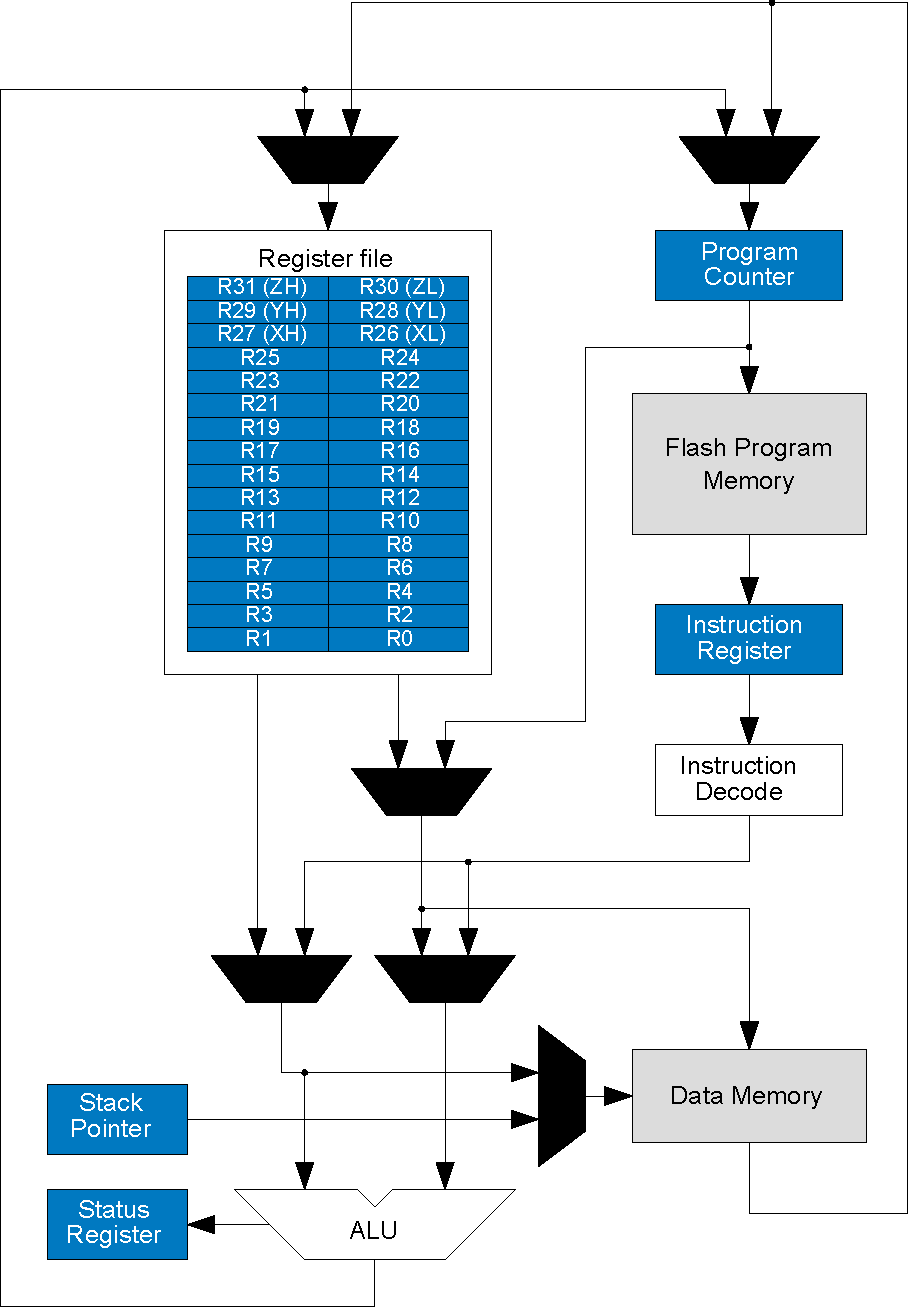
\includegraphics[height = 12cm, keepaspectratio = true]{figures/AVR_CPU.pdf}
    % \caption{} % \label{}
\end{figure}
\subsection{Instructions}
\begin{itemize}
    \item The CPU understands and can execute a limited set of instructions --- \textasciitilde88 unique instructions for the ATtiny1626
    \item Instructions are encoded in programme memory as opcodes. Most instructions are two bytes long, but some instructions are four bytes long
    \item The AVR Instruction Set Manual describes all of the available instructions, and how they are translated into opcodes
    \item Instructions fall loosely into five categories:
          \begin{itemize}
              \item Arithmetic and logic --- ALU
              \item Change of flow --- jumping to different sections of the code or making decisions
              \item Data transfer --- moving data in/out of registers, into the data space, or into RAM
              \item Bit and bit-test --- looking at data in registers (which bits are set or not set)
              \item Control --- changing what the CPU is doing
          \end{itemize}
\end{itemize}
\subsection{Interacting with memory and peripherals}
\begin{itemize}
    \item The CPU interacts with both memory and peripherals via the data space
    \item From the perspective of the CPU, the data space is single large array of
          locations that can be read from, or written to, using an address
    \item We control peripherals by reading from, and writing to, their registers
    \item Each peripheral register is assigned a unique address in the data space
    \item When a peripheral is accessed in this manner we refer to it as being
          memory mapped, as we access them as if they were normal memory
    \item Different devices, peripherals and memory can be included in a memory map
          (and sometimes a device can be accessed at multiple different addresses)
\end{itemize}
\subsection{Memory map}
\begin{figure}[H]
    \centering
    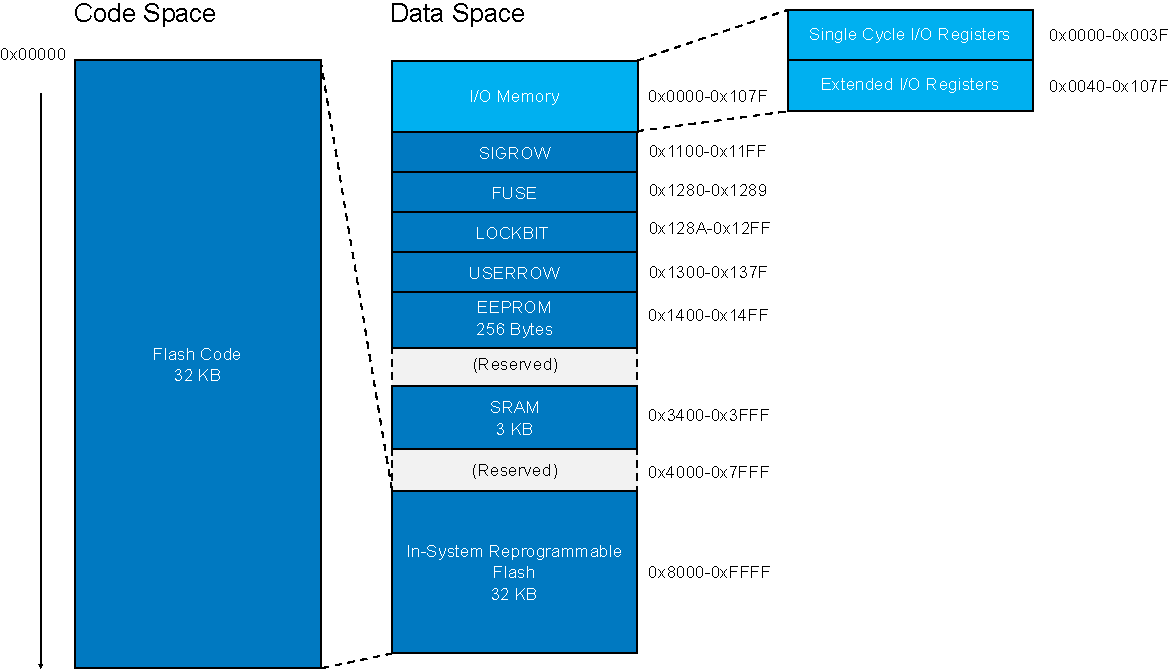
\includegraphics[height = 8cm, keepaspectratio = true]{figures/memory_map.pdf}
    \caption{ATtiny1626 memory map.} % \label{}
\end{figure}
\subsection{Assembly code}
\begin{itemize}
    \item The opcodes placed into programme memory are called
          machine code (i.e., code the machine operates on directly)
    \item We don't write machine code directly as it is:
          \begin{itemize}
              \item Not human readable
              \item Prone to errors (swapping a single bit can completely change the operation)
          \end{itemize}
    \item Instead we can write instructions directly in assembly code
    \item We use instruction mnemonics to specify each instruction:\@ \keywordinline{ldi}, \keywordinline{add}, \keywordinline{sts}, \mintinline{ca65}{jmp}, \dots
    \item An assembler takes assembly code and translates it into opcodes that can
          be loaded into programme memory
\end{itemize}
\section{Digital Representations and Operations}
\subsection{Digital Systems}
A \textbf{bit}\footnote{The term \textit{bit} comes from \textbf{b}inary dig\textbf{it}.}
is the most basic unit of information in a digital system.
A bit encodes a logical state with one of two possible values (i.e., binary).
These states are often referred to as:
\begin{itemize}
    \item true, false
    \item high, low (voltage states)
    \item on, off (logical states)
    \item set, reset
    \item 1, 0
\end{itemize}
A sequence of \textit{eight} bits is known as a \textbf{byte}, and it is the most
common representation of data in digital systems.
A sequence of \textit{four} bits is known as a \textbf{nibble}.

A sequence of \(n\) bits can represent up to \(2^n\) states.
\subsection{Representation}
\subsubsection{Binary Representation}
The \textbf{binary system} is a base-2 system that uses a sequence of bits to represent a number.
Bits are written left-to-right from \textbf{most significant} to \textbf{least significant} bit.

The first bit is the ``most significant'' bit because it is associated with the highest value in the sequence (coefficient of the highest power of two).
\begin{itemize}
    \item The \textbf{least significant bit} (LSB) is at bit index 0.
    \item The \textbf{most significant bit} (MSB) is at bit index \(n - 1\) in an \(n\)-bit sequence.
\end{itemize}
\begin{align*}
    0000_2 & = 0 & 0100_2 & = 4 & 1000_2 & = 8  & 1100_2 = 12 \\
    0001_2 & = 1 & 0101_2 & = 5 & 1001_2 & = 9  & 1101_2 = 13 \\
    0010_2 & = 2 & 0110_2 & = 6 & 1010_2 & = 10 & 1110_2 = 14 \\
    0011_2 & = 3 & 0111_2 & = 7 & 1011_2 & = 11 & 1111_2 = 15
\end{align*}
The subscript 2 indicates that the number is represented using a base-2 system.
\subsubsection{Hexadecimal Representation}
The \textbf{hexadecimal system} (hex) is a base-16 system. As we need 16 digits in this system, we use the letters A to F to represent digits 10 to 15.

Hex is a convenient notation when working with digital systems as each hex digit maps to a nibble.
\begin{align*}
    0_{16} & = 0000_2 & 4_{16} & = 0100_2 & 8_{16} & = 1000_2 & C_{16} = 1100_2 \\
    1_{16} & = 0001_2 & 5_{16} & = 0101_2 & 9_{16} & = 1001_2 & D_{16} = 1101_2 \\
    2_{16} & = 0010_2 & 6_{16} & = 0110_2 & A_{16} & = 1010_2 & E_{16} = 1110_2 \\
    3_{16} & = 0011_2 & 7_{16} & = 0111_2 & B_{16} & = 1011_2 & F_{16} = 1111_2
\end{align*}
\subsubsection{Numeric Literals}
When a fixed value is declared directly in a program, it is referred to as a \textbf{literal}.
Generally, numeric literals can be expressed as either binary, decimal, or hexadecimal, so we
use prefixes to denote various bases. Typically,
\begin{itemize}
    \item \textbf{Binary} notation requires the prefix \mintinline{ca65}{0b}
    \item \textbf{Decimal} notation does not require prefixes
    \item \textbf{Hexadecimal} notation requires the prefix \mintinline{ca65}{0x}
\end{itemize}
For example, \mintinline{ca65}{0x80 |=| 0b10000000 |=| 128}.
\subsection{Unsigned Integers}
The \textbf{unsigned integers} represent the set of counting (natural) numbers, starting at 0.
In the \textbf{decimal system} (base-10), the unsigned integers are encoded using a sequence of decimal digits (0--9).

The decimal system is a \textbf{positional numeral system}, where the contribution of each digit is determined by its position.
For example,
\begin{align*}
    278_{10} & = 2 \times 10^2 &  & + 7 \times 10^1 &  & + 8 \times 10^0 \\
             & = 2 \times 100  &  & + 7 \times 10   &  & + 8 \times 1    \\
             & = 200           &  & + 70            &  & + 8             \\
\end{align*}
In the \textbf{binary system} (base-2) the unsigned integers are encoded using a sequence of binary digits (0--1)
in the same manner. For example,
\begin{align*}
    10101_2 & = 1 \times 2^4 &  & + 0 \times 2^3 &  & + 1 \times 2^2 &  & + 0 \times 2^1 &  & + 1 \times 2^0 \\
            & = 1 \times 16  &  & + 0 \times 8   &  & + 1 \times 4   &  & + 0 \times 2   &  & + 1 \times 1   \\
            & = 16           &  & + 0            &  & + 4            &  & + 0            &  & + 1            \\
            & = 21_{10}
\end{align*}
The range of values an \(n\)-bit binary number can hold when encoding an unsigned integer is 0 to \(2^n - 1\).
\begin{table}[H]
    \centering
    \begin{tabular}{c c}
        \toprule
        \textbf{No.\ of Bits} & \textbf{Range}                        \\
        \midrule
        8                     & \(0\)--\(255\)                        \\
        16                    & \(0\)--\(\num{65535}\)                \\
        32                    & \(0\)--\(\num{4294967295}\)           \\
        64                    & \(0\)--\(\num{18446744073709551615}\) \\
        \bottomrule
    \end{tabular}
    \caption{Range of available values in binary representations.} % \label{}
\end{table}
\subsection{Signed Integers}
Signed integers are used to represent integers that can be positive or negative.
The following representations allow us to encode negative integers using a sequence of binary bits:
\begin{itemize}
    \item Sign-magnitude
    \item One's complement
    \item Two's complement (most common)
\end{itemize}
\subsubsection{Sign-Magnitude}
In sign-magnitude representation, the most significant bit encodes the sign of the
integer. In an 8-bit sequence, the remaining 7-bits are used to
encode the value of the bit.
\begin{itemize}
    \item If the sign bit is 0, the remaining bits represent a positive value,
    \item If the sign bit is 1, the remaining bits represent a negative value.
\end{itemize}
As the sign bit consumes one bit from the sequence, the range of values that can be
represented by an \(n\)-bit sign-magnitude encoded bit sequence is:
\begin{equation*}
    -\left( 2^{n - 1} - 1 \right) \text{ to } 2^{n - 1} - 1
\end{equation*}
For 8-bit sequences, this range is: \(-127\) to \(127\).

However, there are some issues with this representation.
\begin{enumerate}
    \item There are two ways to represent zero: \mintinline{ca65}{0b10000000 |=| 0}, or \mintinline{ca65}{0b00000000 |=| -0}.
    \item Arithmetic and comparison requires inspecting the sign bit
    \item The range is reduced by 1 (due to the redundant zero representation)
\end{enumerate}
\subsubsection{One's Complement}
In one's complement representation, a negative number is represented by
inverting the bits of a positive number (i.e., \(0 \to 1\) and \(1 \to 0\)).

The range of values are still the same:
\begin{equation*}
    -\left( 2^{n - 1} - 1 \right) \text{ to } 2^{n - 1} - 1
\end{equation*}
however, this representation tackles the second problem in the previous representation as
addition is performed via standard binary addition with \textit{end-around carry} (carry bit is added onto result).
\begin{equation*}
    a - b = a + \left( \text{\textasciitilde} b \right) + C.
\end{equation*}
\subsubsection{Two's Complement}
In two's complement representation, the most significant bit encodes a negative weighting of
\(-2^{n - 1}\). For example, in 8-bit sequences, index-7 represents a value of \(-128\).

The two's complement is calculated by adding 1 to the one's complement.

The range of values are:
\begin{equation*}
    -2^{n - 1} \text{ to } 2^{n - 1} - 1
\end{equation*}
This representation is more efficient than the previous because \mintinline{ca65}{0} has a single representation
and subtraction is performed by adding the two's complement of the subtrahend.
\begin{equation*}
    a - b = a + \left( \text{\textasciitilde} b + 1 \right).
\end{equation*}
\subsection{Logical Operators}
\subsubsection{Boolean Functions}
A Boolean function is a function whose arguments and results assume values
from a two-element set, (usually \(\left\{ 0,\: 1 \right\}\) or \mintinline{text}{{false, true}}).

These functions are also referred to as \textit{logical functions} when they operate on bits.
The most common logical functions available to microprocessors and most programming languages are:
\begin{itemize}
    \item Negation: \keywordinline{NOT}
    \item Conjunction: \mintinline{ca65}{AND}
    \item Disjunction: \keywordinline{OR}
    \item Exclusive disjunction: \keywordinline{XOR}
\end{itemize}
By convention, we map a bit value of \mintinline{ca65}{0} to \mintinline{ca65}{false}, and a bit value of \mintinline{ca65}{1} to \mintinline{ca65}{true}.
\subsubsection{Negation}
\mintinline{ca65}{NOT} is a unary operator that is used to \textbf{invert} a bit.
It is typically expressed as:
\begin{itemize}
    \item \keywordinline{NOT} \(a\)
    \item \textasciitilde\(a\)
    \item \(\overline{a}\)
\end{itemize}
Truth table:
\begin{table}[H]
    \centering
    \begin{tabular}{c c}
        \toprule
        \textbf{\(a\)} & \keywordinline{NOT} \(a\) \\
        \midrule
        0              & 1                         \\
        1              & 0                         \\
        \bottomrule
    \end{tabular}
\end{table}
\subsubsection{Conjunction}
\mintinline{ca65}{AND} is a binary operator whose output is true if \textbf{both} inputs are \textbf{true}.
It is typically expressed as:
\begin{itemize}
    \item \(a\) \mintinline{ca65}{AND} \(b\)
    \item \(a\) \mintinline{ca65}{&} \(b\)
    \item \(a \cdot b\)
    \item \(a \land b\)
\end{itemize}
Truth table:
\begin{table}[H]
    \centering
    \begin{tabular}{c c c}
        \toprule
        \textbf{\(a\)} & \textbf{\(b\)} & \textbf{\(a\) \mintinline{ca65}{AND} \(b\)} \\
        \midrule
        0              & 0              & 0                                           \\
        0              & 1              & 0                                           \\
        1              & 0              & 0                                           \\
        1              & 1              & 1                                           \\
        \bottomrule
    \end{tabular}
\end{table}
\subsubsection{Disjunction}
\keywordinline{OR} is a binary operator whose output is true if \textbf{either} input is \textbf{true}.
It is typically expressed as:
\begin{itemize}
    \item \(a\) \keywordinline{OR} \(b\)
    \item \(a\) \mintinline{ca65}{|\vert|} \(b\)
    \item \(a + b\)
    \item \(a \lor b\)
\end{itemize}
Truth table:
\begin{table}[H]
    \centering
    \begin{tabular}{c c c}
        \toprule
        \textbf{\(a\)} & \textbf{\(b\)} & \(a\) \keywordinline{OR} \(b\) \\
        \midrule
        0              & 0              & 0                              \\
        0              & 1              & 0                              \\
        1              & 0              & 1                              \\
        1              & 1              & 1                              \\
        \bottomrule
    \end{tabular}
\end{table}
\subsubsection{Exclusive Disjunction}
\keywordinline{XOR} (Exclusive \keywordinline{OR}) is a binary operator whose output is true if \textbf{only one} input is \textbf{true}.
It is typically expressed as:
\begin{itemize}
    \item \(a\) \keywordinline{XOR} \(b\)
    \item \(a\) \mintinline{ca65}{^} \(b\)
    \item \(a \oplus b\)
\end{itemize}
Truth table:
\begin{table}[H]
    \centering
    \begin{tabular}{c c c}
        \toprule
        \textbf{\(a\)} & \textbf{\(b\)} & \(a\) \keywordinline{XOR} \(b\) \\
        \midrule
        0              & 0              & 0                               \\
        0              & 1              & 1                               \\
        1              & 0              & 1                               \\
        1              & 1              & 0                               \\
        \bottomrule
    \end{tabular}
\end{table}
\subsubsection{Bitwise Operations}
When applying logical operators to a sequence of bits, the operation is performed in a \textbf{bitwise} manner. The result of each operation is stored in the corresponding bit index also.
\subsection{Bit Manipulation}
Often we need to modify individual bits within a byte, \textbf{without} modifying other bits.
This is accomplished by performing a bitwise operation on the byte using a \textbf{bit mask} or \textbf{bit field}.

These operations can:
\begin{itemize}
    \item \textbf{Set} specific bits (change value to \mintinline{ca65}{1})
    \item \textbf{Clear} specific bits (change value to \mintinline{ca65}{0})
    \item \textbf{Toggle} specific bits (change values from \(0 \to 1\), or \(1 \to 0\))
\end{itemize}
\subsubsection{Setting Bits}
To \textbf{set} a bit, we take the bitwise \keywordinline{OR} of the byte, with a bit mask
that has a \textbf{1} in each position where the bit should be set.
\begin{figure}[H]
    \centering
    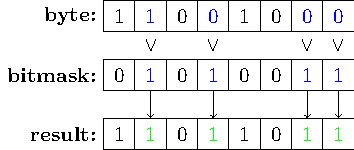
\includegraphics[height = 4cm, keepaspectratio = true]{figures/bit_set.pdf}
    \caption{Setting bits using the logical or.} % \label{}
\end{figure}
\subsubsection{Clearing Bits}
To \textbf{clear} a bit, we take the bitwise \mintinline{ca65}{AND} of the byte, with a bit mask
that has a \textbf{0} in each position where the bit should be cleared.
\begin{figure}[H]
    \centering
    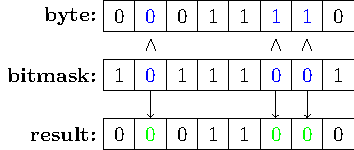
\includegraphics[height = 4cm, keepaspectratio = true]{figures/bit_clear.pdf}
    \caption{Clearing bits using the logical and.} % \label{}
\end{figure}
\subsubsection{Toggling Bits}
To \textbf{toggle} a bit, we take the bitwise \keywordinline{XOR} of the byte, with a bit mask
that has a \textbf{1} in each position where the bit should be toggled.
\begin{figure}[H]
    \centering
    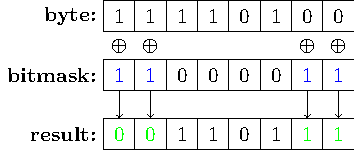
\includegraphics[height = 4cm, keepaspectratio = true]{figures/bit_toggle.pdf}
    \caption{Toggling bits using the logical exclusive or.} % \label{}
\end{figure}
Other bitwise operations act on the entire byte.
\begin{itemize}
    \item One's complement (bitwise \keywordinline{NOT})
    \item Two's complement (bitwise \keywordinline{NOT} + 1)
    \item Shifts
          \begin{itemize}
              \item Logical
              \item Arithmetic (for signed integers)
          \end{itemize}
    \item Rotations
\end{itemize}
\subsubsection{One's Complement}
The one's complement of a byte inverts every bit in the operand. This is done by
taking the bitwise \keywordinline{NOT} of the byte.

Similarly, we can subtract the byte from \mintinline{ca65}{0xFF} to get the one's complement.
\subsubsection{Two's Complement}
The two's complement of a byte is the one's complement of the byte plus one.
Therefore, we can apply take the bitwise \keywordinline{NOT} of the byte, and then add one to it.
\subsubsection{Shifts}
Shifts are used to move bits within a byte. In many programming languages this is represented by two greater than \mintinline{ca65}{>>} or two less than \mintinline{ca65}{<<} characters.
\begin{equation*}
    a \gg s
\end{equation*}
shifts the bits in \(a\) by \(s\) places to the right while adding \mintinline{ca65}{0}'s to the MSB.\
\begin{figure}[H]
    \centering
    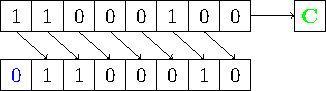
\includegraphics[height = 2cm, keepaspectratio = true]{figures/logical_right_shift.pdf}
    \caption{Right shift using \mintinline{ca65}{lsr} in AVR Assembly.} % \label{}
\end{figure}
Similarly
\begin{equation*}
    a \ll s
\end{equation*}
shifts the bits in \(a\) by \(s\) places to the left while adding \mintinline{ca65}{0}'s to the LSB.\
\begin{figure}[H]
    \centering
    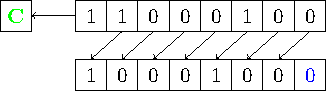
\includegraphics[height = 2cm, keepaspectratio = true]{figures/logical_left_shift.pdf}
    \caption{Left shift using \keyword{\ttfamily{lsl}} in AVR Assembly.} % \label{}
\end{figure}
When using signed integers, the arithmetic shift is used to preserve the value of the sign bit when shifting.
\begin{figure}[H]
    \centering
    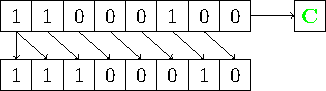
\includegraphics[height = 2cm, keepaspectratio = true]{figures/arithmetic_right_shift.pdf}
    \caption{Arithmetic right shift using \keyword{\ttfamily{asr}} in AVR Assembly.} % \label{}
\end{figure}
Left shifts are used to multiply numbers by 2, whereas right shifts are used to divide numbers by 2 (with truncation).
\subsubsection{Rotations}
Rotatations are used to shift bits with a carry from the previous instruction.
\begin{figure}[H]
    \centering
    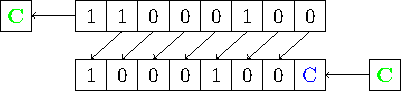
\includegraphics[height = 2cm, keepaspectratio = true]{figures/rotate_left.pdf}
    \caption{Rotate left using \mintinline{ca65}{rol} in AVR Assembly.} % \label{}
\end{figure}
\begin{figure}[H]
    \centering
    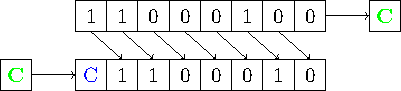
\includegraphics[height = 2cm, keepaspectratio = true]{figures/rotate_right.pdf}
    \caption{Rotate right using \mintinline{ca65}{ror} in AVR Assembly.} % \label{}
\end{figure}
Here the blue bit is carried from the previous instruction, and the carry bit is updated
to the value of the bit that was shifted out.
Rotations are used to perform multi-byte shifts and arithmetic operations.
\subsection{Arithmetic Operations}
\subsubsection{Addition}
Addition is performed using the same process as decimal addition except we only use two digits, 0 and 1.
\begin{enumerate}
    \item \mintinline{ca65}{0b0 + 0b0 = 0b0}
    \item \mintinline{ca65}{0b0 + 0b1 = 0b1}
    \item \mintinline{ca65}{0b1 + 0b1 = 0b10}
\end{enumerate}
When adding two 1's, we carry the result into the next bit position as we would with a 10 in decimal addition.
In AVR Assembly, we can use the \keywordinline{add} instruction to add two bytes. The following
example adds two bytes.
\begin{minted}{ca65}
; Accumulator
|\keyword{ldi}| r16, 0

; First number
|\keyword{ldi}| r17, 29
|\keyword{add}| r16, 17 ; R16 <- R16 + R17 = 0 + 29 = 29

; Second number
|\keyword{ldi}| r17, 118
|\keyword{add}| r16, 17 ; R16 <- R16 + R17 = 29 + 118 = 147
\end{minted}
Below is a graphical illustration of the above code.
\begin{figure}[H]
    \centering
    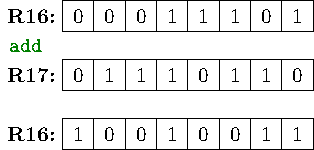
\includegraphics[height = 3cm, keepaspectratio = true]{figures/add.pdf}
    \caption{Overflow addition using \keyword{\ttfamily{add}} in AVR Assembly.} % \label{}
\end{figure}
\subsubsection{Overflows}
When the sum of two 8-bit numbers is greater than 8-bit (255), an \textbf{overflow} occurs.
Here we must utilise a second register to store the high byte so that the result is represented as
a 16-bit number.

To avoid loss of information, a \textbf{carry bit} is used to indicate when an overflow has occurred.
This carry bit can be added to the high byte in the event that an overflow occurs.
This is because the carry bit is 0 when the sum is less than 256, and 1 when the sum is greater than 255.

The following example shows how to use the \mintinline{ca65}{adc} instruction to carry the carry bit when an overflow occurs.
\begin{minted}{ca65}
; Low byte
|\keyword{ldi}| r30, 0
; High byte
|\keyword{ldi}| r31, 0

; Empty byte for adding carry bit
|\keyword{ldi}| r29, 0

; First number
|\keyword{ldi}| r16, 0b11111111
; Add to low byte
|\keyword{add}| r30, r16 ; R30 <- R30 + R16 = 0 + 255 = 255, C <- 0
; Add to high byte
adc r31, r29 ; R31 <- R31 + R29 + C = 0 + 0 + 0 = 0

; Second number
|\keyword{ldi}| r16, 0b00000001
; Add to low byte
|\keyword{add}| r30, r16 ; R30 <- R30 + R16 = 255 + 1 = 0, C <- 1
; Add to high byte
adc r31, r29 ; R31 <- R31 + R29 + C = 0 + 0 + 1 = 1
\end{minted}
Therefore the final result is: \mintinline{ca65}{R31|:|R30 |=| 0b00000001|:|0b00000001 |=| 256}.
Below is a graphical representation of the above code.
\begin{figure}[H]
    \centering
    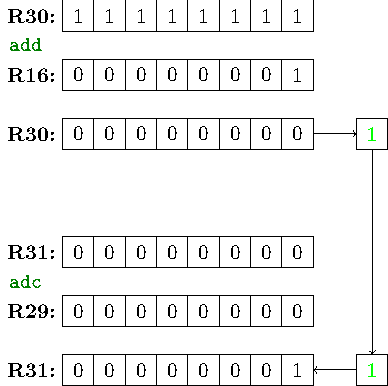
\includegraphics[height = 6cm, keepaspectratio = true]{figures/adc.pdf}
    \caption{Overflow addition using \mintinline{ca65}{adc} in AVR Assembly.} % \label{}
\end{figure}
\subsubsection{Subtraction}
Subtraction is performed using the same process as binary addition, with the
subtrahend in two's complement form.
In the case of overflows, the carry bit is discarded.
\subsubsection{Multiplication}
Multiplication is understood as the sum of a set of partial products, similar to the process used in decimal multiplication.
Here each digit of the multiplier is multiplied to the multipicand and each partial product is added to the result.

Given an \(m\)-bit and an \(n\)-bit number, the product is at most \((m+n)\)-bits wide.
\begin{align*}
    13 \times 43 & = 00001101_2 \times 00101011_2                \\
                 & = \begin{aligned}[t]
                          &   & 00001101_2 &  & \times &  & 1_2      \\
                          & + & 00001101_2 &  & \times &  & 10_2     \\
                          & + & 00001101_2 &  & \times &  & 1000_2   \\
                          & + & 00001101_2 &  & \times &  & 100000_2
                     \end{aligned} \\
                 & = \begin{aligned}[t]
                          &   & 00001101_2  \\
                          & + & 00011010_2  \\
                          & + & 01101000_2  \\
                          & + & 110100000_2
                     \end{aligned}                          \\
                 & = 1000101111
\end{align*}
Using AVR assembly, we can use the \keywordinline{mul} instruction to perform multiplication.
\begin{minted}{ca65}
; First number
|\keyword{ldi}| r16, 13
; Second number
|\keyword{ldi}| r17, 43

; Multiply
|\keyword{mul}| r16, r17 ; R1:R0 <- 0b00000010:0b00101111 = 2:47
\end{minted}
The result is stored in the register pair \mintinline{text}{R1:R0}.
\subsubsection{Division}
Division, square roots and many other functions are very expensive to implement in hardware,
and thus are typically not found in conventional ALUs, but rather
implemented in software.

However, there are other techniques that can be used to implement division in hardware.
By representing the divisor in reciprocal form, we can try to represent the number as
the sum of powers of 2.

For example, the divisor \(6.4\) can be represented as:
\begin{equation*}
    \frac{1}{6.4} = \frac{10}{64} = 10 \times 2^{-6}
\end{equation*}
so that dividing an integer \(n\) by \(6.4\) is approximately equivalent to:
\begin{equation*}
    \frac{n}{6.4} \approx \left( n \times 10 \right) \gg 6
\end{equation*}
When the divisor is not exactly representable as a power of 2 we can use fractional exponents to represent the divisor, however this requires a floating point system implementation which is not provided on the AVR.
\section{Microcontroller Interfacing}
\subsection{Logic Levels}
\subsubsection{Discretisation}
The process of discretisation translates a continuous signal into a discrete signal (bits).
As an example, we can translate \textbf{voltage levels} on microcontroller pins into digital \textbf{logic levels}.
\subsubsection{Logic Levels}
For digital input/output (IO), conventionally:
\begin{itemize}
    \item The voltage level of the positive power supply represents a \textbf{logical 1}, or the \textbf{high state}, and
    \item \qty{0}{V} (ground) represents a \textbf{logical 0}, or the \textbf{low state}.
\end{itemize}
The QUTy is supplied \qty{3.3}{V} so that when a digital output is high,
the voltage present on the corresponding pin will be around \qty{3.3}{V}.
Because voltage is a continuous quantity, we must discretise the full range of voltages into logical levels using \textbf{thresholds}.
\begin{itemize}
    \item A voltage \textbf{above} the input \textbf{high threshold} \(t_H\) is considered \textbf{high}.
    \item A voltage \textbf{below} the input \textbf{low threshold} \(t_L\) is considered \textbf{low}.
\end{itemize}
The interpretation of a voltage between these states is determined by \textbf{hysteresis}.
\subsubsection{Hysteresis}
Hysteresis refers to the property of a system whose state is \textbf{dependent} on
its \textbf{history}. In electronic circuits, this avoids ambiguity in determining
the state of an input as it switches between voltage levels.
\begin{figure}[H]
    \centering
    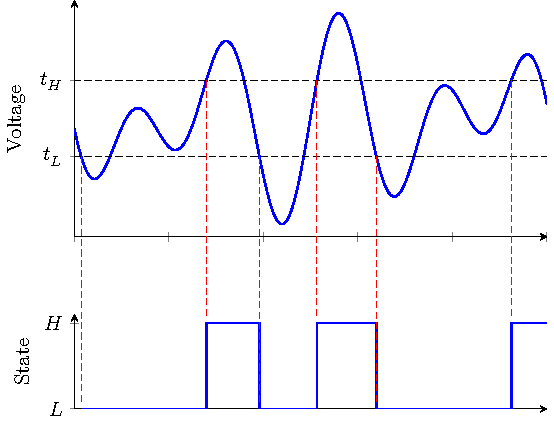
\includegraphics[height = 5cm, keepaspectratio = true]{figures/hysteresis.pdf}
    \caption{Example of hysteresis.} % \label{}
\end{figure}
Given a transition:
\begin{itemize}
    \item If an input is currently in the \textbf{low state}, it has not transitioned to the \textbf{high state} until the voltage crosses the \textbf{high input voltage} threshold.
    \item If an input is currently in the \textbf{high state}, it has not transitioned to the \textbf{low state} until the voltage crosses the \textbf{low input voltage} threshold.
\end{itemize}
It is therefore always preferrable to drive a digital input to an unambiguous voltage level.
\subsection{Electrical Quantities}
\subsubsection{Voltage}
\textbf{Voltage} \(v\) measures the electrical \textit{potential difference} between two points in a circuit, measured in \textbf{Volts (\unit{V})}.
\begin{itemize}
    \item Voltage is measured across a circuit element, or between two points in a circuit, most commonly with respect to a \qty{0}{V} reference (ground).
    \item It represents the \textbf{potential} of the electrical system to do \textbf{work}.
\end{itemize}
\subsubsection{Current}
\textbf{Current} \(i\) measures the \textit{rate of flow of electrical charge} through a circuit, measured in \textbf{Amperes (\unit{A})}.
\begin{itemize}
    \item Current is measured through a circuit element.
\end{itemize}
\subsubsection{Power}
\textbf{Power} \(p\) is the rate of energy transferred per unit time, measured in \textbf{Watts (\unit{W})}.
Power can be determined through the equation
\begin{equation*}
    p = v i.
\end{equation*}
\subsubsection{Resistance}
\textbf{Resistance} \(R\) is a property of a material to \textit{resist the flow of current}, measured in \textbf{Ohms (\unit{\ohm})}.
Ohm's law states that the voltage across a component is proportional to the current that flows through it:
\begin{equation*}
    v = i R.
\end{equation*}
Note that not all circuit elements are resistive (or Ohmic), such that they
do not follow Ohm's law, this can be seen in diodes.
\begin{figure}[H]
    \centering
    \begin{subfigure}{0.47\linewidth}
        \centering
        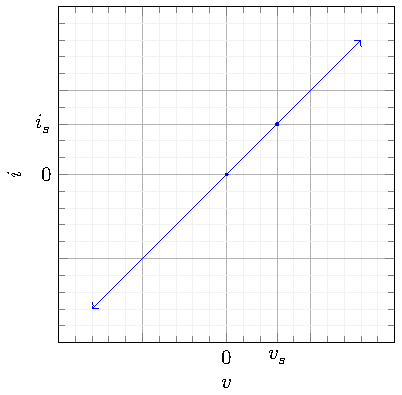
\includegraphics[height=4.5cm]{figures/vi_ohmic.pdf}
        \caption{VI curve for Ohmic components.}
    \end{subfigure}
    \begin{subfigure}{0.47\linewidth}
        \centering
        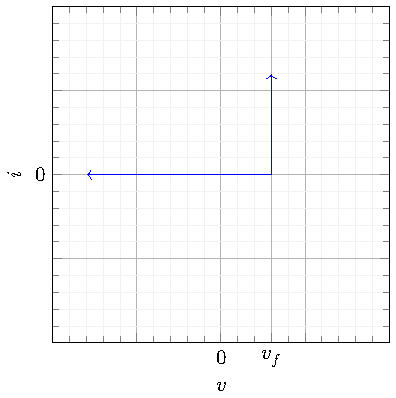
\includegraphics[height=4.5cm]{figures/vi_diode.pdf}
        \caption{VI curve for diodes.}
    \end{subfigure}
    \caption{Voltage-current characteristic curves for various components.}
\end{figure}
Although the wires used to connect a circuit are resistive, we usually assume that they are ideal, that is,
they have zero resistance.
\subsection{Electrical Components}
\subsubsection{Resistors}
A \textbf{resistor} is a circuit element that is designed to have a specific resistance \(R\).
\begin{figure}[H]
    \centering
    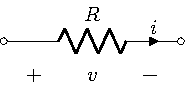
\includegraphics[height = 2.5cm, keepaspectratio = true]{figures/resistor.pdf}
    \caption{Resistor circuit symbol.} % \label{}
\end{figure}
\subsubsection{Switches}
A \textbf{switch} is used to connect and disconnect different elements in a circuit. It can be \textbf{open}
or \textbf{closed}.
\begin{itemize}
    \item In the \textbf{open} state, the switch \textbf{will not conduct}\footnote{Conductance is a measure of the ability for electric charge to flow in a certain path.} current
    \item In the \textbf{closed} state, the switch \textbf{will conduct} current
\end{itemize}
Switches can take a variety of forms:
\begin{itemize}
    \item \textbf{Poles} --- the number of circuits the switch can control.
    \item \textbf{Throw} --- the number of output connections each pole can connect its input to.
    \item Momentary or toggle action
    \item Different form factors, e.g., push button, slide, toggle, etc.
\end{itemize}
Switches are typically for user input.
\begin{figure}[H]
    \centering
    \begin{subfigure}{0.47\linewidth}
        \centering
        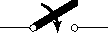
\includegraphics[width=2.5cm]{figures/spst.pdf}
        \caption{Single pole single throw switch.}
    \end{subfigure}
    \begin{subfigure}{0.47\linewidth}
        \centering
        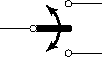
\includegraphics[width=2.5cm]{figures/spdt.pdf}
        \caption{Single pole double throw switch.}
    \end{subfigure}

    \vspace*{5ex}
    \begin{subfigure}{0.47\linewidth}
        \centering
        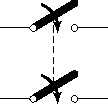
\includegraphics[width=2.5cm]{figures/dpst.pdf}
        \caption{Double pole single throw switch.}
    \end{subfigure}
    \begin{subfigure}{0.47\linewidth}
        \centering
        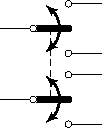
\includegraphics[width=2.5cm]{figures/dpdt.pdf}
        \caption{Double pole double throw switch.}
    \end{subfigure}
    \caption{Various types of switches.}
\end{figure}
\subsubsection{Diodes}
A \textbf{diode} is a semiconductor device that conducts current in
only one direction: from the \textbf{anode} to the \textbf{cathode}.
\begin{figure}[H]
    \centering
    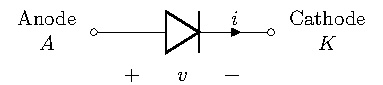
\includegraphics[height = 2cm, keepaspectratio = true]{figures/diode.pdf}
    \caption{Diode symbol.} % \label{}
\end{figure}
Diodes are a non-Ohmic device:
\begin{itemize}
    \item When \textbf{forward biased}, a diode \textbf{does} conduct current, and the anode-cathode voltage
          is equal to the diodes \textbf{forward voltage}.
    \item When \textbf{reverse biased}, a diode \textbf{does not} conduct current, and the cathode-anode voltage
          is equal to the \textbf{applied voltage}.
\end{itemize}
\begin{figure}[H]
    \centering
    \begin{subfigure}{0.47\linewidth}
        \centering
        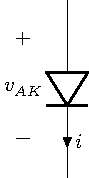
\includegraphics[height=3.5cm]{figures/diode_forward_bias.pdf}
        \caption{Forward biased diode. \\\(v_{AK} = v_f\) and \(i > 0\).}
    \end{subfigure}
    \begin{subfigure}{0.47\linewidth}
        \centering
        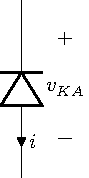
\includegraphics[height=3.5cm]{figures/diode_reverse_bias.pdf}
        \caption{Reverse biased diode. \\\(v_{KA} > 0\) and \(i = 0\).}
    \end{subfigure}
    \caption{Diodes in forward and reverse bias.}
\end{figure}
A diode is only forward biased when the applied anode-cathode voltage \textbf{exceeds} the forward voltage \(v_f\).
A typical forward voltage \(v_f\) for a silicon diode is in the range \qtyrange{0.6}{0.7}{V}, whereas for
Light Emitting Diodes (LEDs), \(v_f\) ranges between \qtyrange{2}{3}{V}.
\subsubsection{Integrated Circuit}
An \textbf{integrated circuit} (IC) is a set of electronic circuits (typically) implemented on a
single piece of semiconductor material, usually silicon. ICs comprise of hundreds to
many thousands of transistors, resistors and capacitors; all implemented on silicon.
ICs are \textbf{packaged}, and connections to the internal circuitry are exposed via \textbf{pins}.

In general, the specific implementation of the IC is not important, but
rather the \textbf{function of the device} and how it \textbf{interfaces} with the rest of the circuit.
Hence ICs can be treated as a functional \textbf{black box}.

For digital ICs:
\begin{itemize}
    \item \textbf{Input pins} are typically \textbf{high-impedance}, and they appear as an open circuit.
    \item \textbf{Output pins} are typically \textbf{low-impedance}, and will actively drive the voltage
          on a pin and any connected circuitry to a \textbf{high} or \textbf{low} state. They can also
          drive connected loads.
\end{itemize}
\subsection{Digital Outputs}
Digital output interfaces are designed to be able to drive connected circuitry to one of states,
high, or low, however, the appropriate technique is \textbf{context specific}.
When referring to digital outputs, we will refer to the states of a net. A \textbf{net}
is defined as the common point of connection of multiple circuit components.

In this section we will consider:
\begin{itemize}
    \item What kind of load the output drives?
    \item Could more than one device be attempting to actively drive the net
          to a specific logic level?
\end{itemize}
\subsubsection{Push-Pull Outputs}
A push-pull digital output is the most common form of output used in digital outputs.
The \textbf{output driver} \(A\) \textit{drives} the \textbf{output state} \(Y\) to:
\begin{itemize}
    \item \textbf{HIGH} by connecting the output net to the supply voltage \(+\unit{V}\).
    \item \textbf{LOW} by connecting the output net to the ground voltage GND (\qty{0}{V}).
\end{itemize}
\begin{figure}[H]
    \centering
    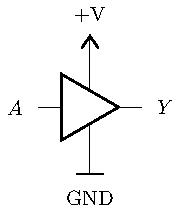
\includegraphics[height = 4cm, keepaspectratio = true]{figures/push_pull.pdf}
    \caption{Push-pull output.} % \label{}
\end{figure}
Hence the output state \(Y\) is determined by the logic level of the output driver \(A\).
\begin{equation*}
    Y = A.
\end{equation*}
\begin{table}[H]
    \centering
    \begin{tabular}{c | c}
        \toprule
        \textbf{\(A\)} & \textbf{\(Y\)} \\
        \midrule
        LOW            & LOW            \\
        HIGH           & HIGH           \\
        \bottomrule
    \end{tabular}
    \caption{Truth table for a push-pull digital output.} % \label{}
\end{table}
The push-pull output \(Y\) can both source and sink current from the connected net.
\subsubsection{High-Impedance Outputs}
In many instances, a digital output is required to be placed in a high-impedance (HiZ) state.
This is accomplished by using an \textbf{output enable} (OE) signal.
\begin{figure}[H]
    \centering
    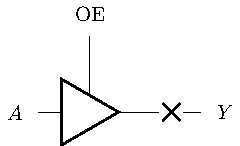
\includegraphics[height = 4cm, keepaspectratio = true]{figures/HiZ.pdf}
    \caption{High-impedance output.} % \label{}
\end{figure}
\begin{itemize}
    \item When the OE signal is \textbf{HIGH}, the output state \(Y\) is determined by the output driver \(A\).
    \item When the OE signal is \textbf{LOW}, the output state \(Y\) is in a \textbf{high-impedance} state.
\end{itemize}
\begin{table}[H]
    \centering
    \begin{tabular}{c c | c}
        \toprule
        \textbf{\(A\)} & \textbf{OE} & \textbf{\(Y\)} \\
        \midrule
        LOW            & LOW         & HiZ            \\
        HIGH           & LOW         & HiZ            \\
        LOW            & HIGH        & LOW            \\
        HIGH           & HIGH        & HIGH           \\
        \bottomrule
    \end{tabular}
    \caption{Truth table for a push-pull digital output.} % \label{}
\end{table}
When the output is in \textbf{HiZ state}:
\begin{itemize}
    \item The output is an effective \textbf{open circuit}, meaning it has \textbf{no effect} on the rest of the circuit.
    \item The voltage on the output net is determined by the \textbf{other circuitry} connected to the net.
\end{itemize}
HiZ outputs are typically used when multiple need to signal over the same wire(s).
\subsubsection{Pull-up and Pull-down Resistors}
When \textbf{no devices} are actively driving a net (e.g., all connected outputs are in the HiZ state),
the state of the net is not well-defined. Hence we can use a \textbf{pull-up} or \textbf{pull-down} resistor
to ensure that the state of the pin is always \textbf{well-defined}.
\begin{multicols}{2}
    \begin{figure}[H]
        \centering
        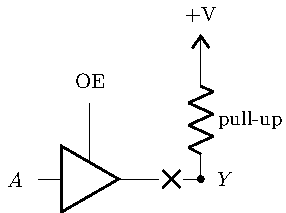
\includegraphics[height = 4cm, keepaspectratio = true]{figures/pullup_resistor.pdf}
        \caption{Pull-up resistor.} % \label{}
    \end{figure}
    \begin{figure}[H]
        \centering
        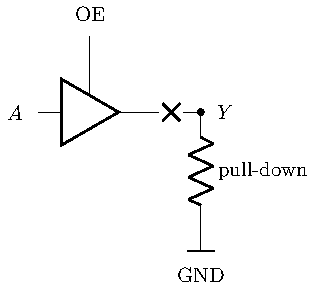
\includegraphics[height = 4cm, keepaspectratio = true]{figures/pulldown_resistor.pdf}
        \caption{Pull-down resistor.} % \label{}
    \end{figure}
\end{multicols}
\begin{itemize}
    \item When \textbf{no circuitry} is actively driving the net, the resistor will passively pull the voltage to either the voltage supply, or ground.
    \item When \textbf{another device} actively drives the net, the active device defines the voltage of the net. Hence the current from the resistor is simply sourced
          or sunk by the \textbf{active device}.
\end{itemize}
The resistors used as pull-up and pull-down resistors are typically in the \unit{k\ohm} range.
\subsubsection{Open-Drain Outputs}
Multiple push-pull outputs should never be connected to the same net
as when one output is driven HIGH and another is driven LOW,
an effective short circuit is created and one or more devices may be damaged.
While push-pull outputs with an output enable may be used,
the timing must be carefully managed.

Hence a more robust solution is to use open-drain outputs.
\begin{figure}[H]
    \centering
    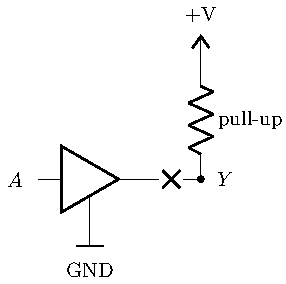
\includegraphics[height = 4cm, keepaspectratio = true]{figures/open_drain.pdf}
    \caption{Open-drain output.} % \label{}
\end{figure}
An open-drain output is either:
\begin{itemize}
    \item In the \textbf{high-impedance} state, where the pull-up resistor is used to pull the net to the \textbf{high state} when the net is \textbf{not driven low}.
    \item \textbf{Connected to ground}, when the net is \textbf{driven low}.
\end{itemize}
\subsection{Microcontroller Pins}
Microcontrollers are interfaced via their exposed pins.
These pins are the only means to access inputs and outputs, and
they are used to interface with other electronic circuits in order to achieve a required functionality.
Pins can be used for:
\begin{itemize}
    \item General purpose input and output (GPIO) --- pin represents a digital state
    \item Peripheral functions
    \item Other functions (power supply, reset input, clock input, etc.)
\end{itemize}
Pins are typically organised into groups of related IO banks,
referred to as \textbf{ports} on the AVR microcontroller.

These ports and pins are assigned an alphanumeric identifier, (e.g., PB7 for pin 7 on port B).
\begin{figure}[H]
    \centering
    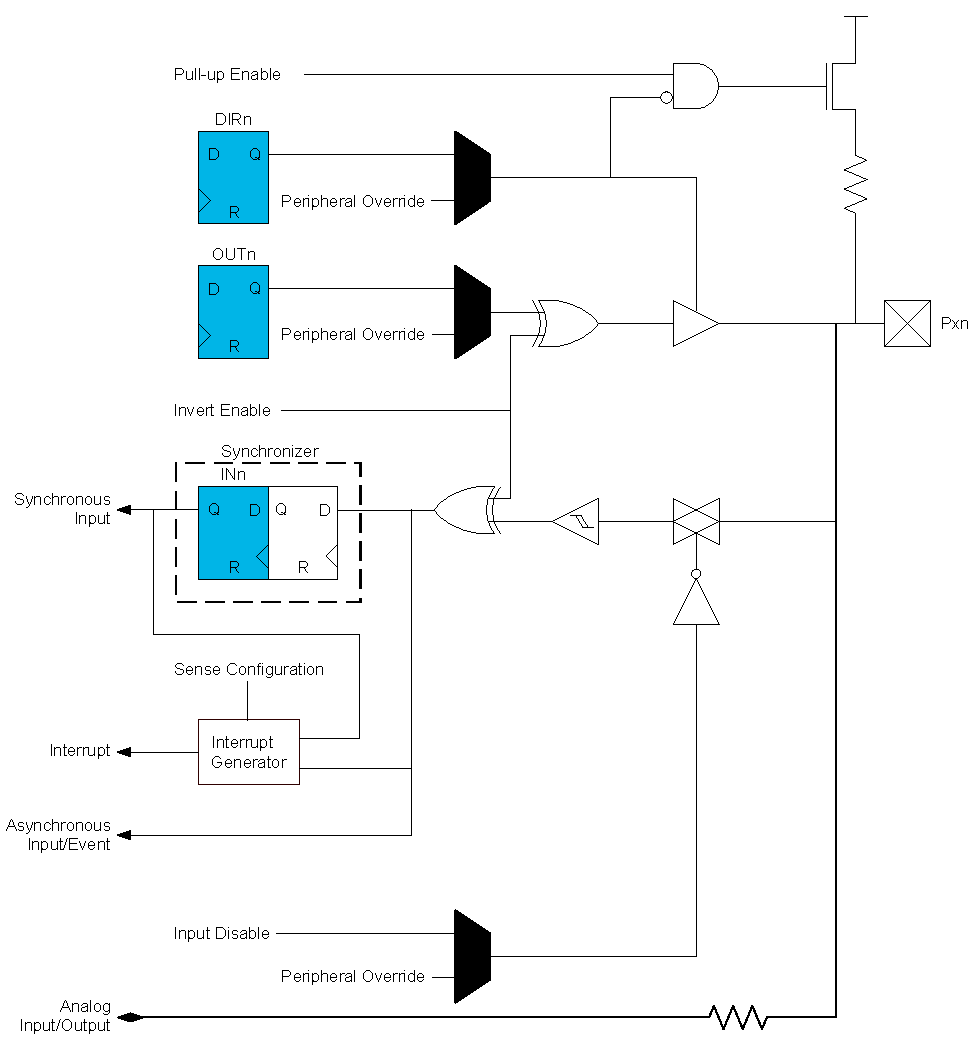
\includegraphics[height = 8cm, keepaspectratio = true]{figures/PORT_block_diagram.pdf}
    \caption{ATtiny1626 PORT block diagram.} % \label{}
\end{figure}
To summarise this diagram:
\begin{itemize}
    \item The data direction register (DIR) controls the push-pull output enable.
    \item The output driver register (OUT) drives the output state.
    \item The input register (IN) reads the output state.
    \item The internal pull-up register enabled through software.
    \item The physical voltage on the pin can be routed to an analogue to digital converter (ADC)
    \item Other peripheral functions can override port pin configurations and the output state.
\end{itemize}
\subsubsection{Configuring an Output in Assembly}
\begin{enumerate}
    \item Place the port pin in a \textbf{safe initial state}
          by writing to the OUT register (HIGH or LOW depending on the context).
    \item Configure the port pin as an output by \textbf{setting} the corresponding bits in the DIR register.
    \item Set the desired pin state by writing to the OUT register.
\end{enumerate}
\begin{minted}{ca65}
; Load macros for easy access to port data space addresses.
\#include <avr/io.h>

; Bitmask for pin 5
|\keyword{ldi}| r16, PIN5_bm

; Set initial safe state
|\keyword{sts}| PORTB_OUTCLR, r16 ; LOW if active HIGH
|\keyword{sts}| PORTB_OUTSET, r16 ; HIGH if active LOW

; Enable output
|\keyword{sts}| PORTB_DIRSET, r16 ; Enable output on PB5

; Set output state to desired value
|\keyword{sts}| PORTB_OUTSET, r16 ; Set state of PB5 to HIGH
\end{minted}
\subsubsection{Configuring an Input in Assembly}
\begin{enumerate}
    \item If required, enable the internal pull-up resistor by \textbf{setting}
          the PULLUPEN bit in the \linebreak corresponding PINnCTRL register.
    \item Read the IN register to get the current state of the pin.
    \item Isolate the relevant pin using the AND operator.
\end{enumerate}
\begin{minted}{ca65}
; Load macros for easy access to port data space addresses.
#include <avr/io.h>

; Bitmask for pin 5
|\keyword{ldi}| r16, PIN5_bm

; Enable internal pull-up resistor if required
|\keyword{sts}| PORTB_PIN5CTRL, r16

; Read output state from data space
|\keyword{lds}| r17, PORTA_IN
; Read output state using virtual PORT
|\keyword{in}| r17, VPORTA_IN

; Isolate desired pin
|\keyword{andi}| r17, r16
\end{minted}
\subsubsection{Peripheral Multiplexing}
Pins can be used to connect internal peripheral functions
to external devices.
As microcontrollers have more peripheral functions than available pins,
peripheral functions are typically multiplexed onto pins.
\begin{definition}[Multiplexing]
    Multiplexing is a method by which \textbf{multiple peripheral} \linebreak \textbf{functions}
    are mapped to the \textbf{same pin}.
    In this scenario, only one function can be enabled at a time, and the pin
    cannot be used for GPIO\@.
\end{definition}
\begin{itemize}
    \item Peripheral functions can be mapped to different \textbf{sets of pins} to provide
          flexibility and to avoid clashes when multiple peripherals are used in
          an application.
    \item When enabled, peripheral functions \textbf{override} standard port functions.
    \item The \textbf{Port Multiplexer} (PORTMUX) is used to select which
          \textbf{pin set} should be used by a peripheral.
    \item Certain peripherals can have their inputs/outputs mapped to different
          \textbf{sets of pins} through the PORTMUX\@.
\end{itemize}
Note that we cannot re-map a single peripheral function to another pin, but must consider the entire set.
\subsection{Interfacing to Simple IO}
\subsubsection{Driving LEDs}
The \textbf{brightness} of an LED is proportional to the \textbf{current}
passing through it. As LEDs are non-Ohmic, we cannot drive them directly
with a voltage as this would result in an uncontrolled flow of current that
may damage the LED or driver.

Instead, LEDs are paired with a \textbf{series resistor} to limit the flow of current.
The appropriate current is dependent on the specific LED that is used
and the capability of the driver device (microcontroller).
A typical indictor LED requires a current of \qtyrange{1}{2}{m.A}.
\subsubsection{Interfacing to LEDs}
An LED can be driven in two different configurations from a microcontroller pin:
\begin{itemize}
    \item \textbf{active high}; in which case the LED is \textbf{lit} when the pin is \textbf{HIGH}.
    \item \textbf{active low}; in which case the LED is \textbf{lit} when the pin is \textbf{LOW}.
\end{itemize}
Both of these configurations have their benefits, and the best configuration depends entirely on the context.
\pagebreak
\begin{multicols}{2}
    \begin{figure}[H]
        \centering
        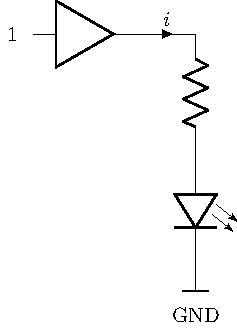
\includegraphics[height = 4cm, keepaspectratio = true]{figures/active_high_LED.pdf}
        \caption{LED in an active high configuration.} % \label{}
    \end{figure}
    \begin{figure}[H]
        \centering
        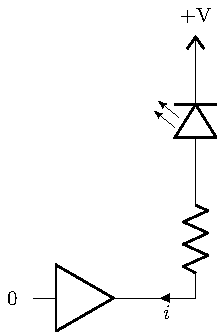
\includegraphics[height = 4cm, keepaspectratio = true]{figures/active_low_LED.pdf}
        \caption{LED in an active low configuration.} % \label{}
    \end{figure}
\end{multicols}
On the QUTy, the LED display is driven in the \textbf{active low} configuration.
This has a number of advantages:
\begin{itemize}
    \item If the internal pull-up resistors are mistakenly enabled, no current will
          flow into the LEDs.
    \item The microcontroller pins can sink higher currents than they can source,
          allowing us to drive the display to a higher brightness.
    \item The display used on the QUTy has a common anode configuration, hence we must use an
          active low configuration to drive the display segments independently.
\end{itemize}
An LED is an example of a simple \textbf{digital output}, as we can map \textbf{logical states}
to \textbf{LED states} (lit or unlit) for a digital output.
\subsubsection{Switches as Digital Inputs}
The state of a switch can be used to \textbf{set} the state of a pin.
As the switch has two states (open or closed), these can be mapped directly to
\textbf{logical states}.

This can be done by connecting the switch between the pin and voltage source
representing one of the logic levels (ground or a positive supply).
\begin{multicols}{2}
    \begin{figure}[H]
        \centering
        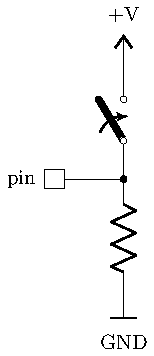
\includegraphics[height = 5cm, keepaspectratio = true]{figures/active_high_switch.pdf}
        \caption{Switch in an active high \\ configuration.} % \label{}
    \end{figure}
    \begin{figure}[H]
        \centering
        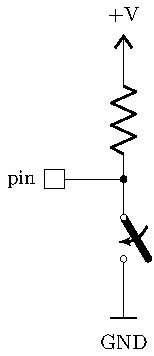
\includegraphics[height = 5cm, keepaspectratio = true]{figures/active_low_switch.pdf}
        \caption{Switch in an active low configuration.} % \label{}
    \end{figure}
\end{multicols}
\begin{itemize}
    \item When the switch is \textbf{open}, the pull-up/pull-down resistor is used to define the state of the switch.
    \item When the switch is \textbf{closed}, the state of the pin is defined by the voltage connected to via the switch.
\end{itemize}
\subsubsection{Interfacing to Switches}
As with LEDs, we can interface switches to microcontroller pins in two different configurations:
\begin{itemize}
    \item \textbf{active high}; in which case the pin is \textbf{HIGH} when the switch is \textbf{closed}.
    \item \textbf{active low}; in which case the pin is \textbf{LOW} when the switch is \textbf{closed}.
\end{itemize}
An \textbf{active low} configuration is usually preferred as:
\begin{itemize}
    \item it allows for the utilisation of an \textbf{internal pull-up resistor} that is commonly
          implemented in microcontrollers.
    \item It eliminates the risk of unsafe voltages being applied to the pin from the power supply in an active high configuration.
    \item It is easier to access a ground reference on a circuit board.
\end{itemize}
\subsubsection{Interfacing to Integrated Circuits}
For digital ICs,
\begin{itemize}
    \item \textbf{Inputs} are typically \textbf{high impedance}
    \item \textbf{Outputs} are typically \textbf{push-pull}
\end{itemize}
This generally means that we can interface an IC by connecting its pins directly to the pins of a microcontroller.
\begin{itemize}
    \item For \textbf{IC inputs}, the microcontroller pin is configured as an \textbf{output},
          and the \textbf{microcontroller sets} the logic level of the net.
    \item For \textbf{IC outputs}, the microcontroller pin is configured as an \textbf{input},
          and the \textbf{IC sets} the logic level of the net.
\end{itemize}
As microcontroller pins are typically configured as \textbf{inputs on reset}, a
pull-up/pull-down resistor may be required if it is important for an IC input to
have a \textbf{known state} prior to the configuration of the relevant microcontroller pins as outputs.
\section{Assembly Programming}
\begin{definition}[Word]
    A word refers to a value that is two bytes in size (16-bit).
\end{definition}
\subsection{Registers}
A register refers to a memory location that is 1 byte in size (8-bit).
The ATtiny1626 has 32 registers of which \mintinline{ca65}{r16} to \mintinline{ca65}{r31} can be loaded with an immediate value (\numrange{0}{255}) using \keywordinline{ldi}.
\begin{minted}{ca65}
|\keyword{ldi}| r16, 17
|\keyword{ldi}| r19, 0b10101010
|\keyword{ldi}| r31, 0xFF
\end{minted}
Values are commonly loaded into registers as many other operations can be performed on them.
\subsection{Flow Control}
Instructions on the AVR Core increment the PC by 1 or 2 (depending on whether the OPCODE is 1 or 2 words) when they are executed so that any successive
instructions are executed after the first. To divert execution to a different location, we can utilise
\textbf{change of flow} instructions. The AVR Core has many change of flow instructions, that each have a different
effect on the execution of the program.

The \mintinline{ca65}{jmp} (jump) instruction is used the simplest to jump to a different location in the program.
This instruction is capable of jumping to an address withtin the entire 4M (words) program memory, however,
this is highly excessive for the ATtiny1626.
\subsection{Labels}
Most change of flow instructions take an \textbf{address} in program memory as a parameter.
Hence to make this process easier, we can use labels to refer to locations in program memory (and also RAM).
\begin{minted}{ca65}
entry:
    |\keyword{ldi}| r16, 0
    jmp new_location ; Jump to the label |\textbf{new\_location}|.
    |\keyword{ldi}| r16, 1 ; This instruction is skipped

; Label
new_location:
    |\keyword{push}| r16
\end{minted}
When a label appears in source code, the assembler replaces references to it with the address of the
directive/instruction immediately following that label. Labels work for both \textbf{absolute} and \textbf{relative}
addresses and the assembler will automatically adjust the address to the correct type.

Additionally, labels can also be used as parameters to other immediate instructions if we store the high and low
bytes in registers and wish to reference the location in an indirect jumping instruction.
\subsection{Absolute and Relative Addresses}
\mintinline{ca65}{jmp} is a 32-bit instruction, which uses 22 bits to specify an address between \mintinline{ca65}{0x000000}
and \mintinline{ca65}{0x3FFFFF}, or \(2^{23} - 1\) bits of memory (\qty{8}{MB}). As mentioned earlier, this is much larger
than what the 16-bit PC can address on the ATtiny1626 (\qty{64}{KB}).

As we will only need to jump within \qty{64}{KB} of memory, it is inefficient to use the \mintinline{ca65}{jmp} instruction as it
requires 3 CPU cycles to execute. Therefore, many AVR change of flow instructions take a value that is
\textbf{added} onto the current PC to calculate the destination address, allowing them to fit within 16 bits.

The \keywordinline{rjmp} (relative jump) instruction works in the same manner as the absolute jump instruction. It only requires 2
CPU cycles and because the assembler calculates the relative address locations, we do not need to determine the relative distances.

Note the assembler throw an error if the address is not within the range of the PC\@.
\subsection{Branching}
A branching instruction jumps to a different location in response to something that occurs, i.e., user input, internal state, or other external factors.
Many change of flow instructions are conditional, and will alter the PC differently based on register value(s) or flags.
In AVR there are two main categories of branching instructions:
\begin{itemize}
    \item Branch instructions
    \item Skip instructions
\end{itemize}
\subsubsection{Branch Instructions}
Branch instructions use the following logic:
\begin{enumerate}
    \item Check if the specified flag in SREG is cleared/set
    \item If true, jump to the specified address (\(\mathrm{PC} \leftarrow \mathrm{PC} + k + 1\))
    \item Otherwise, proceed to the next instruction as normal (\(\mathrm{PC} \leftarrow \mathrm{PC} + 1\))
\end{enumerate}
Although there are are 20 branch instructions listed in the instruction set summary, the following two form the basis of all branching instructions:
\begin{itemize}
    \item \keywordinline{brbc} (branch if bit in SREG is cleared)
    \item \keywordinline{brbs} (branch if bit in SREG is set)
\end{itemize}
All other branching instructions are specific cases of the above instructions, that are provided to make programming in Assembly easier.
As these instructions check the bits in the SREG, they are usually preceded by an ALU operation such as \keywordinline{cp} or \keywordinline{cpi} to trigger the required flags.

As only 7 bits are allocated to the destination in the OPCODE, branch instructions jump shorter distances than relative jumps.
\subsubsection{Compare Instructions}
Both the \keywordinline{cp} and \keywordinline{cpi} instructions are used to compare the values in one or two registers.
The ALU performs a subtraction operation whose result is used to update the SREG\@. Note that the result is not stored or used in any way.
\begin{itemize}
    \item \mintinline{ca65}{|\keyword{cp}| Rd, Rr} performs \mintinline{ca65}{Rd} \(-\) \mintinline{ca65}{Rr}
    \item \mintinline{ca65}{|\keyword{cpi}| Rd, K} performs \mintinline{ca65}{Rd} \(-\) \mintinline{ca65}{K}
\end{itemize}
Note \keywordinline{cp} compares the values in two registers, whereas \keywordinline{cpi} compares the value in a register with an immediate value.
The result of this operation is used to set the appropriate flags in the SREG.
\begin{minted}{ca65}
entry:
    |\keyword{ldi}| r16, 0
    |\keyword{ldi}| r19, 10
    |\keyword{cp}| r16, r19 ; Compare values in registers r16 and r19
    |\keyword{brge}| new_location ; Branch if r16 greater than or equal to r19

new_location:
\end{minted}
Note that many instructions are able to set the Z flag, which is used to indicate if the result of the operation is zero.
In these cases, the compare instruction may be redundant.
\subsubsection{Skip Instructions}
The skip instructions are less flexible then branch instructions, but can sometimes require less space or fewer cycles.
Skip instructions skip the next instruction if the condition is true.

In this example we will skip the line which increments register 16.
\begin{minted}{ca65}
|\keyword{cpse}| r16, r17 ; Skips next instruction if r16 == r17
inc r16 ; This is skipped

|\keyword{push}| r16 ; PC is now here
\end{minted}
Same example which uses a branch instruction:
\begin{minted}{ca65}
entry:
    |\keyword{cp}| r16, r17
    |\keyword{breq}| new_location ; Skips to new_location if r16 == r17
    inc r16 ; This is skipped

new_location:
    |\keyword{push}| r16 ; PC is now here
\end{minted}
Note that the number of cycles for a skip instruction depend on the size of the instruction being skipped.

The \keywordinline{sbrc} and \keywordinline{sbrs} instructions are used to skip the next instruction if the specified bit a register is cleared/set.
\begin{minted}{ca65}
|\keyword{ldi}| r16, 0b00101110

|\keyword{sbrc}| r16, 0 ; Skips next instruction if bit 0 of r16 is cleared
inc r16 ; This is skipped

|\keyword{push}| r16 ; PC is now here
\end{minted}
Comparing with branch instructions
\begin{minted}{ca65}
entry:
    |\keyword{ldi}| r16, 0b00101110

    |\keyword{andi}| r16, 0b00000001 ; Isolate bit 0

    |\keyword{breq}| new_location ; Skips next instruction if r16 == 0
    inc r16 ; This is skipped

new_location:
    |\keyword{push}| r16 ; PC is now here
\end{minted}
The \keywordinline{sbis} and \keywordinline{sbic} instructions are used to skip the next instruction if the specified bit an I/O register is set/cleared.
For example, if we wish to toggle the decimal point LED (DISP DP) on the QUTy (PORT B pin 5) when the first button (BUTTON0) was pressed (PORT A pin 4),
\begin{minted}{ca65}
|\keyword{ldi}| r16, PIN5_bm ; Bitmask of pin 5
|\keyword{sbis}| VPORTA_IN, 0b00010000 ; Skip next instruction if pin 4 of PORT A is set
|\keyword{sts}| PORTB_OUTTGL, r16 ; Toggle the output driver of pin 5 on PORT B
\end{minted}
Using branch instructions:
\begin{minted}{ca65}
entry:
    |\keyword{in}| r17, VPORTA_IN ; Read the input register of PORT A
    |\keyword{andi}| r17, 0b00010000 ; Isolate pin 4

    |\keyword{brne}| new_location ; Skip instructions if r17 != 0

    |\keyword{ldi}| r16, PIN5_bm ; Bitmask of pin 5
    |\keyword{sts}| PORTB_OUTTGL, r16 ; Toggle the output driver of pin 5 on PORT B

new_location:
\end{minted}
\subsection{Loops}
By jumping to an earlier address, we can loop over a block of instructions.
\begin{minted}{ca65}
infinite_loop:
    ; Code to repeat

    |\keyword{rjmp}| infinite_loop
\end{minted}
Loops can also be finite, in which case the loop will terminate when a counter reaches zero.
\begin{minted}{ca65}
|\keyword{ldi}| r16, 10 ; Set counter to 10

loop:
    dec r16 ; Decrement counter
    |\keyword{brne}| loop ; Branch if counter != 0
\end{minted}
Loops can also be used to repeat until some external event occurs.
\begin{minted}{ca65}
main_loop:
    |\keyword{in}| r17, VPORTA_IN ; Read the input register of PORT A
    |\keyword{andi}| r17, 0b00010000 ; Isolate pin 4

    |\keyword{brne}| main_loop ; Branch if counter != 0

    |\keyword{rjmp}| button_pressed

button_pressed:
    ; Execute instructions

    |\keyword{rjmp}| main_loop ; Return to main loop
\end{minted}
\subsection{Delays}
Loops can be utilised to delay the execution of instructions. These instructions do
not execute any useful code. This is useful for when we wish to wait for an external event to occur.\footnote{Note that this type of loop is not recommended for time-sharing systems, such as a personal computer, as the lost CPU cycles cannot be used by other programs. In these cases, clock interrupts are preferred. However, on a device such as the ATtiny1626, delay loops can be utilised to precisely insert delays in a program.}

To create a precisely timed delay, we must take the following values into account.
\begin{itemize}
    \item The clock speed --- frequency of the clocks oscillations (default: \qty{20}{MHz} --- configurable in CLKCTLR\_MCLKCTRLA)
    \item The prescaler --- reduces the frequency of the CPU clock through division by a specific amount; 12 different settings from 1x to 64x (default: 6 --- configurable in CLKCTLR\_MCLKCTRLA)
\end{itemize}
The clock oscillates at its effective clock speed:
\begin{equation*}
    \text{effective clock speed} = \text{clock speed} \times \frac{1}{\text{prescaler}}
\end{equation*}
The default prescaler is 6, so the effective clock speed is \qty{3.33}{MHz} by default.
Note that the effective clock speed can therefore range between:
\begin{itemize}
    \item Effective maximum clock frequency: \qty{20}{MHz} (\qty{20}{MHz} clock \& prescaler 1)\footnote{As the QUTy is supplied with \qty{3.3}{V}, it is not safe to go above \qty{10}{MHz}.}
    \item Effective minimum clock frequency: \qty{512}{Hz} (\qty{32.768}{kHz} clock \& prescaler 64)
\end{itemize}
Therefore to create a delay, we must first determine the required number of CPU cycles in the body of the loop
and iterate until the number of CPU cycles reaches the required amount.

The following examples utilise counters of various sizes to create delays.
Note that \(n\) represents the number of iterations.
\begin{minted}{ca65}
delay_1:
    |\keyword{ldi}| r16, 255 - n ; 1 CPU cycle

    ; Incrementor
    |\keyword{ldi}| r17, 1 ; 1 CPU cycle

    loop:
        add r16, r17 ; 1 CPU cycle
        |\keyword{brcc}| loop ; 2 CPU cycles (1 CPU cycle when condition is false)
\end{minted}
The total number of CPU cycles is:
\begin{align*}
    \text{total cycles} & = 1 + 1 + \left( n + 1 \right) + 2 n + 1 \\
                        & = 3 n + 4
\end{align*}
for a maximum delay of \qty{230.7}{\micro s} (\(\left( 3 \times \left( 2^8 - 1 \right) + 4 \right) T\))\footnote{\(T\) is the period of one CPU cycle (using the default clock configuration): \(T = \frac{1}{\qty{20}{MHz} / 6} = \qty{300}{ns}\).}.
To create larger delays, we can use multiple registers:
\begin{minted}{ca65}
delay_2:
    |\keyword{ldi}| r24, x ; 1 CPU cycle
    |\keyword{ldi}| r25, y ; 1 CPU cycle

    loop:
        |\keyword{adiw}| r24, 1 ; 2 CPU cycles
        |\keyword{brcc}| loop ; 2 CPU cycles (1 CPU cycle when condition is false)
\end{minted}
The register pair \(\left( y:x \right)\) has the following relationship:
\begin{align*}
    \left( y:x \right) = \left( 2^{17} - 1 \right) - n \iff n = \left( 2^{17} - 1 \right) - \left( y:x \right)
\end{align*}
with
\begin{align*}
    \text{total cycles} & = 1 + 1 + 2 \left( n + 1 \right) + 2 n + 1 \\
                        & = 4n + 5
\end{align*}
for a maximum delay of \qty{78.644}{ms} (\(\left(4 \times \left( 2^{16} - 1 \right) + 5 \right) T\)).
With three registers,
\begin{minted}{ca65}
delay_3:
    |\keyword{ldi}| r24, x ; 1 CPU cycle
    |\keyword{ldi}| r25, y ; 1 CPU cycle
    |\keyword{ldi}| r26, z ; 1 CPU cycle

    loop:
        |\keyword{adiw}| r24, 1 ; 2 CPU cycles
        |\keyword{adc}| r26, r0 ; 1 CPU cycle (r0 represents a register with value 0)
        |\keyword{brcc}| loop ; 2 CPU cycles (1 CPU cycle when condition is false)
\end{minted}
The register triplet \(\left( z:y:x \right)\) is determined through:
\begin{align*}
    \left( z:y:x \right) = \left( 2^{25} - 1 \right) - n \iff n = \left( 2^{25} - 1 \right) - \left( z:y:x \right)
\end{align*}
with
\begin{align*}
    \text{total cycles} & = 1 + 1 + 1 + 2 \left( n + 1 \right) + \left( n + 1 \right) + 2 n + 1 \\
                        & = 5n + 7
\end{align*}
for a maximum delay of \qty{25.166}{s} (\(\left(5 \times \left( 2^{24} - 1 \right) + 7 \right) T\)).
This approach can be extended to create delays of any length.

If needed, we can also include the \mintinline{ca65}{nop} (no operation) instruction which requires 1 CPU cycle and does nothing.
In addition to this, we can also utilise nested loops, however the timing is more complex to determine.
\subsection{Memory and IO}
On the AVR Core, as both I/O and SRAM are accessed through the data space, they can be
directly accessed using instructions that read/write to memory. This approach is known as memory-mapped I/O (MMIO)
and it significantly reduces chip complexity.

In contrast to modern CPU architectures, such as x86, in the AVR architecture,
programs are located in a separate address space (although the memory is still accessible through the data space).
\begin{figure}[H]
    \centering
    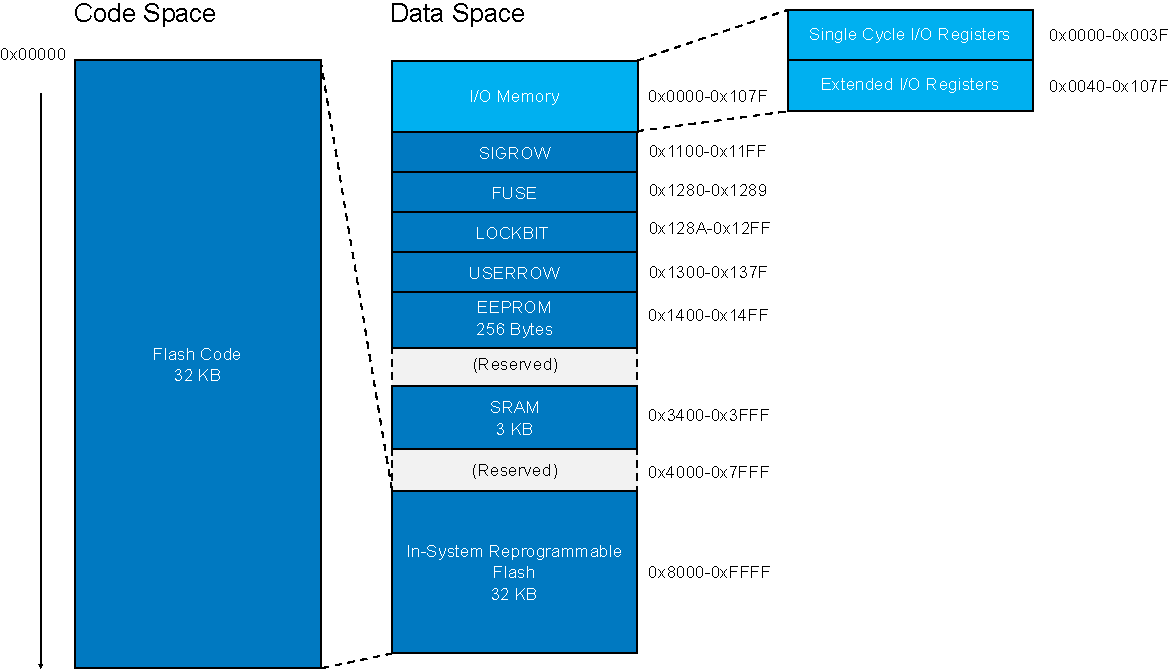
\includegraphics[height = 8cm, keepaspectratio = true]{figures/memory_map.pdf}
    \caption{ATtiny1626 memory map.} % \label{}
\end{figure}
The following instructions may be used to access memory from the data space:
\begin{itemize}
    \item \keywordinline{lds} (load direct from data space to register)
    \item \keywordinline{sts} (store direct from register to data space)
    \item \keywordinline{ld} (load indirect from data space to register)
    \item \keywordinline{st} (store indirect from register to data space)
    \item \keywordinline{push}/\keywordinline{pop} (stack operations)
    \item \keywordinline{in}/\keywordinline{out} (single cycle I/O register operations)
    \item \keywordinline{sbi}/\keywordinline{cbi} (set/clear bit in I/O register)
\end{itemize}
Note that the \keywordinline{in}/\keywordinline{out} instructions can
only access the low 64 bytes of the I/O register space and the \keywordinline{sbi}/\keywordinline{cbi}
instructions can only access the low 32 bytes of the I/O register space.

As the name suggests, these instructions only require a single CPU cycle and hence
several \linebreak VPORT\{A, B, C\} (virtual ports) addresses are mapped to this location, so that they can be
accessed through these single cycle instructions.

VPORT addresses simply hold a copy of their corresponding PORTs.
\subsubsection{Load/Store Indirect}
Although the \keywordinline{lds}/\keywordinline{sts} instructions can be used to access exact addresses
of bytes, they are generally not suitable for accessing data structures such as arrays.

Instead, the \keywordinline{ld}/\keywordinline{st} instructions allow transfers between
registers and the data space, where addresses are stored in a pointer register.
These pointer registers are available for use only by \keywordinline{ld}/\keywordinline{st}
through \keywordinline{X}, \keywordinline{Y}, and \keywordinline{Z}.

These 16-bit pointer registers occupy the same space as registers \mintinline{ca65}{r26} to \mintinline{ca65}{r31}.
\begin{itemize}
    \item \mintinline{ca65}{r26} \(\to\) \keywordinline{XL} (\keywordinline{X}-register low byte)
    \item \mintinline{ca65}{r27} \(\to\) \keywordinline{XH} (\keywordinline{X}-register high byte)
    \item \mintinline{ca65}{r28} \(\to\) \keywordinline{YL} (\keywordinline{Y}-register low byte)
    \item \mintinline{ca65}{r29} \(\to\) \keywordinline{YH} (\keywordinline{Y}-register high byte)
    \item \mintinline{ca65}{r30} \(\to\) \keywordinline{ZL} (\keywordinline{Z}-register low byte)
    \item \mintinline{ca65}{r31} \(\to\) \keywordinline{ZH} (\keywordinline{Z}-register high byte)
\end{itemize}
For example, if we wanted to access a byte in RAM, we can do the following:
\begin{minted}{ca65}
; Store address of RAM in X
|\keyword{ldi}| XL, lo8(RAMSTART)
|\keyword{ldi}| XH, hi8(RAMSTART)

|\keyword{ld}| r16, X ; Load byte from X to r16
; The byte in X is now in r16

|\keyword{ldi}| r17, 24
|\keyword{st}| X, r17 ; Store byte from r16 to X
; The byte in X is now 24
\end{minted}
These pointer registers also support post-increment and pre-decrement operations:
\begin{itemize}
    \item \mintinline{ca65}{X+} (post-increment pointer address)
    \item \mintinline{ca65}{-X} (pre-decrement pointer address)
\end{itemize}
\begin{minted}{ca65}
|\keyword{ld}| r16, X+ ; Load byte from X to r16, then X <- X + 1
|\keyword{st}| X+, r16 ; Store byte from r16 to X, then X <- X + 1

|\keyword{ld}| r16, -X ; X <- X - 1, then load byte from X to r16
|\keyword{st}| -X, r16 ; X <- X - 1, then store byte from r16 to X
\end{minted}
This operation can be used to copy bytes from one location to another:
\begin{minted}{ca65}
; Copy 10 bytes from RAM to RAM+10
|\keyword{ldi}| XL, lo8(RAMSTART)
|\keyword{ldi}| XH, hi8(RAMSTART)

|\keyword{ldi}| YL, lo8(RAMSTART+10)
|\keyword{ldi}| YH, hi8(RAMSTART+10)

|\keyword{ldi}| r16, 10 ; Loop 10 times
loop:
    |\keyword{ld}| r0, X+ ; Load byte from X to r0, then X <- X + 1
    |\keyword{st}| Y+, r0 ; Store byte from r0 to Y, then Y <- Y + 1
    dec r16
    |\keyword{brne}| loop
\end{minted}
\subsubsection{Load/Store Indirect with Displacement}
In addition to the \keywordinline{ld}/\keywordinline{st} instructions, the \keywordinline{ldd}/\keywordinline{std}
instructions are a special form that allow us to load/store from/to the address of the pointer register
\textbf{plus} \(q = \left\{ \numrange{0}{63} \right\}\).
\begin{minted}{ca65}
|\keyword{ldi}| YL, lo8(RAMSTART)
|\keyword{ldi}| YH, hi8(RAMSTART)

|\keyword{ldd}| r0, Y+20 ; Load byte from Y+20 to r0
|\keyword{std}| Y+21, r0 ; Store byte from r1 to Y+21
; Note Y still points to RAMSTART
\end{minted}
Note this form is only available for \keywordinline{Y}, and \keywordinline{Z}.
\subsection{Stack}
The stack is a last-in first-out (LIFO) data structure in SRAM\@.
It is accessed through a register called the stack pointer (SP),
which is not part of the register file like SREG\@.

Upon reset, SP is set to the last available address in SRAM (\mintinline{ca65}{0x3FFF}),
and can be modified through \keywordinline{push}/\keywordinline{pop} and other methods that are generally not recommended.
\begin{itemize}
    \item \keywordinline{push} stores a register to SP then decrements SP (\(\mathrm{SP} \leftarrow \mathrm{SP} - 1\))
    \item \keywordinline{pop} increments SP (\(\mathrm{SP} \leftarrow \mathrm{SP} + 1\)) then loads to a register from SP
\end{itemize}
If a particular register is required without modifying other code, we can temporarily
store the value of that register on the stack, and pop it back when we are done:
\begin{minted}{ca65}
; Temporarily store Z on the stack
|\keyword{push}| ZL
|\keyword{push}| ZH

; Z may be used for another purpose

; Restore Z from the stack
|\keyword{pop}| ZH
|\keyword{pop}| ZL
\end{minted}
Notice that the values are popped in reverse order.
\subsection{Procedures}
Procedures allow us to write modular, reusable code which makes them powerful when working on
complex projects. Although they are usually associated with high level languages as
methods, or functions, they are also available in assembly.

Procedures begin with a label, and end with the \mintinline{ca65}{ret} keyword.
They must be \textbf{called} using the \keywordinline{call}/\keywordinline{rcall} instructions.
\begin{minted}{ca65}
procedure:
    ; Procedure body
    |\keyword{ret}| ; Return to caller
\end{minted}
\subsubsection{Saving Context}
To ensure that procedures are maximally flexible and place no constraints on the caller,
we must always restore any modified registers before returning to the caller. The same is
true for the SREG\@.
\begin{minted}{ca65}
|\keyword{rjmp}| main_loop

procedure:
    |\keyword{push}| r16 ; Save r16 on the stack

    ; Procedure body
    ; Code that modifies r16
    |\keyword{ldi}| r16, 0x12
    loop:
        dec r16
        |\keyword{brne}| loop

    |\keyword{pop}| r16 ; Restore r16 from the stack
    |\keyword{ret}|

main_loop:
    |\keyword{ldi}| r16, 10
    |\keyword{rcall}| procedure ; Call procedure

    |\keyword{push}| r16 ; r16 should still be 10
\end{minted}
\subsubsection{Parameters and Return Values}
Parameters can be passed using registers or the stack depending on the size of
the inputs.
\begin{minted}{ca65}
|\keyword{rjmp}| main_loop

; Calculate the average of two numbers
; Inputs:
;     r16: first number
;     r17: second number
; Outputs:
;     r16: average
average:
    ; Save r0
    |\keyword{push}| r0

    ; Save SREG
    |\keyword{in}| r0, CPU_SREG
    |\keyword{push}| r0

    ; Calculate average
    |\keyword{add}| r16, r17
    ror r16

    ; Restore SREG
    |\keyword{pop}| r0
    |\keyword{out}| CPU_SREG, r0

    ; Restore r0
    |\keyword{pop}| r0

    ; Return
    |\keyword{ret}|

main_loop:
    ; Arguments
    |\keyword{ldi}| r16, 100
    |\keyword{ldi}| r17, 200

    ; Call procedure
    |\keyword{rcall}| average
\end{minted}
Using the stack:
\begin{minted}{ca65}
|\keyword{rjmp}| main_loop

; Calculate the average of two numbers
; Inputs:
;     top two values on stack
; Outputs:
;     r16: average
average:
    ; Save Z
    |\keyword{push}| ZL
    |\keyword{push}| ZH

    ; Save SREG
    |\keyword{in}| ZL, CPU_SREG
    |\keyword{push}| ZL

    ; Get SP location
    |\keyword{in}| ZL, CPU_SPL
    |\keyword{in}| ZH, CPU_SPH

    ; Save r17
    |\keyword{push}| r17

    ; Get first number
    |\keyword{ldd}| r16, Z+7
    ; Get second number
    |\keyword{ldd}| r17, Z+6

    ; Calculate average
    |\keyword{add}| r16, r17
    ror r16

    ; Restore r17
    |\keyword{pop}| r17

    ; Restore SREG
    |\keyword{pop}| ZL
    |\keyword{out}| CPU_SREG, ZL

    ; Restore Z
    |\keyword{pop}| ZH
    |\keyword{pop}| ZL

    ; Return
    |\keyword{ret}|

main_loop:
    ; Arguments
    |\keyword{ldi}| r16, 100
    |\keyword{push}| r16
    |\keyword{ldi}| r16, 200
    |\keyword{push}| r16

    ; Call procedure
    |\keyword{rcall}| average

    ; Remove arguments from the stack
    |\keyword{pop}| r0
    |\keyword{pop}| r0
\end{minted}
Note that it is preferrable to return values using registers.
\section{C Programming}
C is a programming language developed in the early 1970s by Dennis Richie.
C is a compiled language, meaning that a separate program is used to
efficiently translate the source code into assembly.
Its compilers are capable of targetting a wide variety of microprocessor architectures
and hence it is used to implement all major operating system kernels.
Compared to many other languages, C is a very efficient programming
language as its constructs map directly onto machine instructions.
\subsection{Introduction}
\subsubsection{Main Function}
C is a procedural language and hence all code subsides in a procedure (known as a \textbf{function}).
In C, the \mintinline{c}{main} function is the \textbf{entry point} to the program.
Program execution will generally begin in this function, where we can make calls to other functions.
\begin{minted}{c}
int main()
{
    // Function body
    return 0;
}
\end{minted}
The purpose of returning a zero at the end of the \mintinline{c}{main} function
is to signify the \textbf{exit status code} of the process. An exit status of \mintinline{c}{0} is traditionally
used to indicate success, while all non-zero values indicate failure.
\subsubsection{Statements}
C programs are made up of statements. Statements are placed within scopes (indicated by braces (\mintinline{c}{{}}))
and are executed in the order they are placed. All statements in C must terminate with a semicolon (\mintinline{c}{;}).
Although assembly instructions translate to a single OPCODE, a single C statement can translate to multiple OPCODEs.
\begin{minted}{c}
int main()
{
    int x = 3;
    {
        int y = 4;
        x = x + y;
    }
    // x is now 7
    // y is no longer in scope
    return 0;
}
\end{minted}
\subsubsection{Comments}
C supports two styles of comments. The first of these are known as ``C-style comments'', which
allow multi-line/block comments. Multi-line comments use the \mintinline{c}{/* */} syntax.
\begin{minted}{c}
/*
    This is a multi-line comment.
    It can span multiple lines.
*/
\end{minted}
The second style is known as ``C++-style comments'', which allow single-line comments.
These comments are denoted by the \mintinline{c}{//} syntax.
\begin{minted}{c}
// This is a single-line comment.
int x = 3; // It can be placed after a statement.
\end{minted}
All comments in C are ignored by the compiler.
\section{Variables}
Variables are used to temporarily store values in memory.
Variables have a \textbf{type} and a \textbf{name} and must be declared before use.
\subsection{Declaration}
To declare a variable in C, we must specify the type and name of that variable.
\begin{minted}{c}
int x;
\end{minted}
This variable can then be \textbf{assigned to} using the \mintinline{c}{=} operator.
\begin{minted}{c}
x = 4;
\end{minted}
\subsection{Initialisation}
To optionally assign a value during declaration, we can apply the assignment operator after
the declaration. This is known as a variable \textbf{initialisation}, as we are assigning an initial value to the variable.
\begin{minted}{c}
int x = 4;
\end{minted}
Note that using \textbf{uninitialised variables} results in \textbf{unspecified behaviour} in C, meaning that
the value of such variables is unpredictable.
\subsection{Types}
While AVR assembly supports 8-bit registers, C supports larger data types by treating them as a sequence of bytes.
We can also create compound data types with \mintinline{c}{struct} and \mintinline{c}{union}.
\subsubsection{Type Specifiers}
Type specifiers in declarations define the type of the variable.
The \mintinline{c}{signed char}, \mintinline{c}{signed int}, and
\mintinline{c}{signed short int}, \mintinline{c}{signed long int} types, together with their \mintinline{c}{unsigned} variants
and \mintinline{c}{enum}, are all known as \textbf{integral} types.
\mintinline{c}{float}, \mintinline{c}{double}, and \mintinline{c}{long double} are known as \textbf{floating} or \textbf{floating-point} types.
Arithmetic between

The following table summarises various numeric types in C\@:
\begin{table}[H]
    \centering
    \begin{tabular}{c c c}
        \toprule
        \textbf{Description}           & \textbf{Size} & \textbf{Equivalent Definitions}                              \\
        \midrule
        Character data                 & \qty{1}{B}    & \mintinline{c}{signed char c; char c;}                       \\
        Signed short                   & \qty{2}{B}    & \mintinline{c}{signed short int s; signed short s; short s;} \\
        Unsigned short                 & \qty{2}{B}    & \mintinline{c}{unsigned short int us; unsigned short us;}    \\
        Signed integer                 & \qty{4}{B}    & \mintinline{c}{signed int i; signed i; int i;}               \\
        Unsigned integer               & \qty{4}{B}    & \mintinline{c}{unsigned int ui; unsigned ui;}                \\
        Signed long                    & \qty{8}{B}    & \mintinline{c}{signed long int l; signed long l; long l;}    \\
        Unsigned long                  & \qty{8}{B}    & \mintinline{c}{unsigned long int ul; unsigned long ul;}      \\
        Single precision floating      & \qty{4}{B}    & \mintinline{c}{float f;}                                     \\
        Double precision floating      & \qty{8}{B}    & \mintinline{c}{double d;}                                    \\
        Long double precision floating & \qty{16}{B}   & \mintinline{c}{long double ld;}                              \\
        \bottomrule
    \end{tabular}
    % \caption{} % \label{}
\end{table}
Note that the size of these types is not necessarily the same across platforms, hence it is discouraged to use these keywords for
platform specific tasks. \emph{See the section on \hyperref[sec:exact_width_types]{Exact Width Types} for more information}.
\subsubsection{Type Qualifiers}
Types can be qualified with additional keywords to modify the properties of
the identifier. Three common qualifiers are \textbf{const}, \textbf{static}, and \textbf{volatile}.
\begin{itemize}
    \item \mintinline{c}{const} --- indicates that the variable is \textbf{constant} and cannot be modified.
    \item \mintinline{c}{static} --- indicates that the variable has a global lifetime (maintains value between function invocations).
    \item \mintinline{c}{volatile} --- indicates that the variable can be modified or accessed by other programs or hardware.
\end{itemize}
\subsubsection{Portable Types}
C has a set of standard types that are defined in the language specification,
however the type specifiers shown above may have different storage sizes depending on the platform.
Although this may be insignificant for most platforms, microcontrollers
use specific sizes for registers, meaning it is important to refer to the correct
type specifiers when declaring a variable.
\subsubsection{Exact Width Types}\label{sec:exact_width_types}
The standard integer (\mintinline{c}{stdint.h}) library provides \textbf{exact-width} type definitions that are specific to
the development platform. This ensures that variables can be initialised with the correct size on any platform.
\begin{minted}{c}
#include <stdint.h>

int main()
{
    int8_t i8;
    int16_t i16;
    int32_t i32;
    int64_t i64;

    uint8_t ui8;
    uint16_t ui16;
    uint32_t ui32;
    uint64_t ui64;

    return 0;
}
\end{minted}
\subsubsection{Floating-Point Types}
The \mintinline{c}{float} and \mintinline{c}{double} types can store \textbf{floating-point} value types in C.
Their implementation allows for variable levels of precision, i.e., extremely large and extremely small values.
These types are very useful on systems with a floating point unit (FPU) or equivalent.

As the ATtiny1626 does not have an FPU, arithmetic involving floating point values is highly inefficient. Therefore,
integer arithmetic should be utilised when possible. Note that a single floating point number or operation causes
the entire floating point library to be included which can require a large amount of memory.
\section{Literals}
\subsection{Integer Prefixes}
Integer literals are assumed to be base 10 unless a prefix is specified. C supports
all of the following prefixes:
\begin{itemize}
    \item \textbf{Binary} (base 2) --- \mintinline{c}{0b}
    \item \textbf{Octal} (base 8) --- \mintinline{c}{0}
    \item \textbf{Decimal} (base 10) --- no prefix
    \item \textbf{Hexadecimal} (base 16) --- \mintinline{c}{0x}
\end{itemize}
\subsection{Integer Suffixes}
Integer literals can be suffixed to specify the size/type of the value:
\begin{itemize}
    \item \textbf{Unsigned} --- \mintinline{c}{U}
    \item \textbf{Long} --- \mintinline{c}{L}
    \item \textbf{Long Long} --- \mintinline{c}{LL}
\end{itemize}
Suffixes are generally only required when clarifying ambiguity of values where the user wishes to use a different type than the default type.
\begin{minted}{c}
#include <stdio.h>

int main()
{
    printf("%d\n", 2147483648); // Treated as signed integer and throws warning
    printf("%d\n", 2147483648U); // Treated as unsigned integer

    return 0;
}
\end{minted}
\subsection{Floating Point Suffixes}
As with integer types, floating point values can also be suffixed to specify which type to use.
\begin{itemize}
    \item \textbf{Float} --- \mintinline{c}{f}
    \item \textbf{Double} --- \mintinline{c}{d}
\end{itemize}
\subsection{Character and String Literals}
\begin{itemize}
    \item \textbf{Character} --- surrounded by single quotes \mintinline{c}{'A'}
    \item \textbf{String} --- surrounded by double quotes \mintinline{c}{"Hello World"}
\end{itemize}
\subsection{Flow Control}
\subsubsection{If Statements}
C provides a standard branching control structure known as an \mintinline{c}{if} statement.
This structure tests a condition and executes a block of code if that condition is \textbf{true}.
\begin{minted}{c}
if (condition)
{
    // Code to execute if condition is true
}
\end{minted}
This structure can be nested and also supports \mintinline{c}{else} and \mintinline{c}{else if} statements.
\begin{minted}{c}
if (x > 1)
{
    // Code to execute if x is greater than 1
    if (x < 10)
    {
        // Code to execute if x is greater than 1 and less than 10
    }
} else if (x < -1)
{
    // Code to execute if x is less than -1
    if (x > -10)
    {
        // Code to execute if x is less than -1 and greater than -10
    }
} else
{
    // Code to execute if x is not greater than 1 and not less than -1
}
\end{minted}
\subsubsection{While Loops}
The simplest loop structure in C is achieved by using a \mintinline{c}{while} loop.
This loop executes a block of code while the condition is \textbf{true}.
\begin{minted}{c}
while (condition)
{
    // Code to execute while condition is true
}
\end{minted}
An \mintinline{c}{do} while loop is similar to a \mintinline{c}{while} loop, but the loop will execute at least once.
\begin{minted}{c}
do
{
    // Code to execute at least once
} while (condition);
\end{minted}
This loop structure is typically accompanied by a looping variable known as an iterator:
\begin{minted}{c}
int i = 0; // Iterator

// Execute code 10 times
while (i < 10)
{
    // Code to execute while i is less than 10

    i++; // Increment i by 1
}
\end{minted}
\subsubsection{For Loops}
\mintinline{c}{for} loops are similar to \mintinline{c}{while} loops, but they usually result in more understandable code.
\begin{minted}{c}
for (initialisation; condition; increment)
{
    // Code to execute while condition is true
}
\end{minted}
Note the initialisation and increment statements are optional, and while the condition statement is also optional,
we must ensure that the loop can terminate from within the structure (see next section).
\subsubsection{Break and Continue Statements}
\mintinline{c}{break} and \mintinline{c}{continue} statements are used to terminate a loop early.
\begin{minted}{c}
for (int i = 0; i < 10; i++)
{
    if (i == 5)
    {
        break; // Terminate loop early
    }
    printf("%d\n", i);
}
\end{minted}
\begin{minted}{c}
for (int i = 0; i < 10; i++)
{
    if (i == 5)
    {
        continue; // Skip current iteration and continue with next iteration
    }
    printf("%d\n", i);
}
\end{minted}
If the loop is nested within another loop, the \mintinline{c}{break} and \mintinline{c}{continue} statements will only terminate the innermost loop.
\begin{minted}{c}
for (int i = 0; i < 10; i++)
{
    for (int j = 0; j < 10; j++)
    {
        if (j == 5)
        {
            break; // Terminate inner loop early
        }
        printf("%d\n", j);
    }
}
\end{minted}
\subsection{Expressions}
C provides a number of operators which can be used to perform arithmetic/logical operations on values.
C follows the same precedence rules as mathematics, however caution should be used when
comparing precedence of certain logical and bitwise operations.
\subsubsection{Operation Precedence}
\setminted{escapeinside={?*}{*?}}
\begin{table}[H]
    \centering
    \begin{tabular}{c c c}
        \toprule
        \textbf{Operation}            & \textbf{Operator Symbol}                                                                                                                                                          & \textbf{Associativity}         \\
        \midrule
        Postfix                       & \mintinline{c}{++}, \mintinline{c}{--}                                                                                                                                            & \multirow{5}{*}{Left to right} \\
        Function call                 & \mintinline{c}{()}                                                                                                                                                                &                                \\
        Array subscripting            & \mintinline{c}{[]}                                                                                                                                                                &                                \\
        Member access                 & \mintinline{c}{.}                                                                                                                                                                 &                                \\
        Member access through pointer & \mintinline{c}{->}                                                                                                                                                                &                                \\
        \midrule
        Prefix                        & \mintinline{c}{++}, \mintinline{c}{--}                                                                                                                                            & \multirow{7}{*}{Right to left} \\
        Unary                         & \mintinline{c}{+}, \mintinline{c}{-}                                                                                                                                              &                                \\
        Logical NOT and bitwise NOT   & \mintinline{c}{!}, \mintinline{c}{~}                                                                                                                                              &                                \\
        Type cast                     & \mintinline{c}{(type)}                                                                                                                                                            &                                \\
        Dereference                   & \mintinline{c}{*}                                                                                                                                                                 &                                \\
        Address-of                    & \mintinline{c}{&}                                                                                                                                                                 &                                \\
        Size-of                       & \mintinline{c}{sizeof}                                                                                                                                                            &                                \\
        \midrule
        Multiplicative                & \mintinline{c}{*}, \mintinline{c}{/}, \mintinline{c}{%}                                                                                                                           & Left to right                  \\
        Additive                      & \mintinline{c}{+}, \mintinline{c}{-}                                                                                                                                              & Left to right                  \\
        Bitwise shift                 & \mintinline{c}{<<}, \mintinline{c}{>>}                                                                                                                                            & Left to right                  \\
        Relational                    & \mintinline{c}{<}, \mintinline{c}{>}, \mintinline{c}{<=}, \mintinline{c}{>=}                                                                                                      & Left to right                  \\
        Equality                      & \mintinline{c}{==}, \mintinline{c}{!=}                                                                                                                                            & Left to right                  \\
        Bitwise AND                   & \mintinline{c}{&}                                                                                                                                                                 & Left to right                  \\
        Bitwise XOR                   & \mintinline{c}{^}                                                                                                                                                                 & Left to right                  \\
        Bitwise OR                    & \mintinline{c}{|}                                                                                                                                                                 & Left to right                  \\
        Logical AND                   & \mintinline{c}{&&}                                                                                                                                                                & Left to right                  \\
        Logical OR                    & \mintinline{c}{||}                                                                                                                                                                & Left to right                  \\
        Conditional                   & \mintinline{c}{? :}                                                                                                                                                               & Right to left                  \\
        Assignment                    & \mintinline{c}{=}, \mintinline{c}{+=}, \mintinline{c}{-=}, \mintinline{c}{*=}, \mintinline{c}{/=}, \mintinline{c}{%=}, \mintinline{c}{&=}, \mintinline{c}{^=}, \mintinline{c}{|=} & Right to left                  \\
        Sequential evaluation         & \mintinline{c}{,}                                                                                                                                                                 & Left to right                  \\
        \bottomrule
    \end{tabular}
    % \caption{} % \label{}
\end{table}
\subsubsection{Arithmetic Operations}
All arithmetic operations work as expected, noting that integer division is truncated.

If an arithmetic operation causes a type overflow, the result will depend on the type.
For signed integers, the result of an overflow is \textbf{undefined} in C. For unsigned integers,
the result is truncated to the type size (or the value modulo the type size).
\subsubsection{Operator Types}
\begin{itemize}
    \item \textbf{Unary} operators --- have a single operand. For example, \mintinline{c}{++} and \mintinline{c}{--}, or \mintinline{c}{+} and \mintinline{c}{-}.
    \item \textbf{Binary} operators --- have two operands. For example, \mintinline{c}{+}, \mintinline{c}{-}, \mintinline{c}{*}, and \mintinline{c}{/}.
    \item \textbf{Ternary} operators --- have three operands. For example, \mintinline{c}{? :}.
\end{itemize}
\subsubsection{Assignment}
To assign a value to a variable, use the assignment (\mintinline{c}{=}) operator.
\begin{minted}{c}
int x = 5;
\end{minted}
\subsubsection{Multiple Assignment}
If we want to assign values to multiple variables of the same type, we can use the comma (\mintinline{c}{,}) operator.
\begin{minted}{c}
int x = 1, y = 2, z = 3;
\end{minted}
We can also use the assignment (\mintinline{c}{=}) operator to assign the same value to multiple variables of the same type.
\begin{minted}{c}
int x, y, z;
x = y = z = 5;
\end{minted}
\subsubsection{Compound Assignment}
Compound assignment operators perform the operation specified by the additional operator,
then assign the result to the left operand.
\begin{minted}{c}
char x = 0b11001010;
x |= 0b00000001; // x = 0b11001010 | 0b00000001 = 0b11001011

int y = 25;
y += 5; // y = 25 + 5 = 30

char z = 0b10000010;
z <<= 1; // z = 0b10000010 << 1 = 0b00000100
\end{minted}
\subsubsection{Bitwise Operations}
Binary operators behave as expected in C.
\begin{minted}{c}
char x = 0b11001010;
unsigned char y = 0b01100001;

char a = ~x;     // a = ~0b11001010 = 0b00110101
char b = x & y;  // b = 0b11001010 & 0b01100001 = 0b01000000
char c = x | y;  // c = 0b11001010 | 0b01100001 = 0b11101011
char d = x ^ y;  // d = 0b11001010 ^ 0b01100001 = 0b10101011

char e = x << 1; // e = 0b11001010 << 1 = 0b10010100
char f = x >> 1; // f = 0b11001010 >> 1 = 0b11100101
char g = y >> 1; // g = 0b01100001 >> 1 = 0b00110000
\end{minted}
Note that right shifts are automatically sign-extended in C.
\subsubsection{Relational Operations}
Relational operators can be used to compare two values.
\begin{minted}{c}
int x = 5;
int y = 10;
int z = 15;

if (x < y) {
    printf("x is less than y\n");
}

if (x != 15)
{
    printf("x is not equal to 15\n");
}
\end{minted}
\subsubsection{Logical Operations}
Logical operators can be used to combine two boolean expressions.
\begin{minted}{c}
int x = 5;
int y = 10;
int z = 15;

if (x < y && x != 15) {
    printf("x is less than y and x is not equal to 15\n");
}
\end{minted}
\subsection{Preprocessor}
The preprocessor processes C code before it is passed onto the compiler.
The preprocessor strips out comments, handles \textbf{preprocessor directives}, and replaces macros.
Preprocessors begin with the \mintinline{c}{#} character and no non-whitespace characters can
appear on the line before the preprocessor directive.
\subsubsection{Includes}
The \mintinline{c}{#include} directive is used to include the contents of another file into the current file.
This directive has two forms.
\begin{itemize}
    \item \mintinline{c}{#include <filename>} --- include header files for the C standard library and other header files associated with the target platform.
    \item \mintinline{c}{#include "filename"} --- include programmer-defined header files that are typically in the same directory as the file containing the directive.
\end{itemize}
When this directive is used, it is equivalent to copying the contents of the file into the current file,
at the location of the directive. The included file is also preprocessed and may contain other include directives.
\subsubsection{Header Files}
Object files containing \textbf{compiled code} can be linked into a program to allow programmers to
call existing functions. For C to have knowledge of the functions in this object file,
the authors of those functions should store the function prototypes in a \textbf{header file}.

Header files end in the \mintinline{text}{.h} extension.
They can be included into the source file using the \mintinline{c}{#include} directive and can significantly
reduce compile times by reducing the amount of code that needs to be compiled.

In the following example, we will define an \mintinline{c}{add} function and include
it into another C program.
\begin{minted}{c}
// add.c
int add(int x, int y)
{
    return x + y;
}
\end{minted}
This file is compiled to \mintinline{text}{add.o}. To allow the \mintinline{c}{add} function to be called from the main program,
we need to create a header file containing the function prototype of \mintinline{c}{add}.
\begin{minted}{c}
// add.h
int add(int x, int y);
\end{minted}
We can then include this header file into the main program.
\begin{minted}{c}
// main.c
#include <stdio.h> // Include printf definition
#include "add.h" // Include add function definition

int main()
{
    int x = 5;
    int y = 10;

    int z = add(x, y);
    printf("%d\n", z);

    return 0;
}
\end{minted}
\subsubsection{Definitions}
The \mintinline{c}{#define} directive is used to define \textbf{preprocessor macros}.
Whenever these macros appear in the source file, they are replaced with the value specified by the macro.
Macros are a simple text replacement mechanism, an thus must be defined carefully to avoid
invalid code from being generated.
\begin{minted}{c}
#include <stdio.h>
#define PI 3.14159265358979

int main()
{
    printf("%f\n", 2 * PI);
    return 0;
}
\end{minted}
Aside from constant values, macros can also be used to create small compile-time ``functions'',
that expand to code:
\begin{minted}{c}
#include <stdio.h>
#define MAX(x, y) ((x) > (y) ? (x) : (y))

int main()
{
    int x = 5;
    int y = 10;

    int z = MAX(x, y);
    printf("%d\n", z);

    return 0;
}
\end{minted}
Note that the semi-colon is omitted at the end of the macro definition,
as it would also be substituted into the program.

Only a single preprocessor directives can appear on a line, and the directives
must occupy a single line (note that a backslash (\mintinline{c}{\}) can be used to break long lines).
\end{document}
